\documentclass{article}

\usepackage{enumerate}

\usepackage{amsmath}

\usepackage{amssymb}

\usepackage{graphicx}

\usepackage{subfigure}

\usepackage{geometry}

\usepackage{color}

\usepackage{bm}

\usepackage{indentfirst}

\usepackage{array}

\usepackage{multirow}
\usepackage{float}
\usepackage{diagbox}
\begin{document}
\hrulefill
\thispagestyle{empty}



\begin{center}

\begin{large}

\sc{UM--SJTU Joint Institute \vspace{0.3em} \\ Physics Laboratory \\(VE215)}

\end{large}



\hrulefill



\vspace*{5cm}

\begin{Large}

\sc{{Laboratory Report}}

\end{Large}



\vspace{2em}



\begin{large}

\sc{{Exercise 5

\vspace{0.5em}



Filter Lab

}}

\end{large}

\end{center}





\vfill



\begin{table}[h!]

\flushleft

\begin{tabular}{lll}

Name: Xu Yiyang \hspace*{2em}&

ID: 518370910020\hspace*{2em}\\





\\



Date: 13 Nov 2019 



\end{tabular}

\end{table}



\newpage
\section{Goal}

\begin{enumerate}

\item

Learn about four types of filters – Low-Pass, High-Pass, Band-Pass, and Band-reject.

\item

Learn about transfer functions.

\item

Predict the theoretical result and make comparison with lab data.

\end{enumerate}
\section{Introduction}

\subsection{Filter}

Filters are everywhere in our lives. The circuits built to operate on signals usually apply filters. For example, telephone lines pass the sounds at frequencies between about 100Hz and 3kHz and practically blocks all other frequencies.

\subsection{Transfer function}

Mathematically, the transfer function is used to analyze what the circuit did to the signal:

$$Transfer\ function=\frac{Output\ signal}{Input\ signal}$$

This function can also be expressed as

$$H(\omega)=\frac{V_{out}(\omega)}{V_{in}(\omega)}$$

The magnitude of the transfer function is called “voltage gain”, often measured as the ratio of the peak-to-peak (ppk) voltages:

$$|H(\omega)|=\left|\frac{V_{out}(\omega)}{V_{in}(\omega)}\right|=\frac{V_{out,ppk}(\omega)}{V_{in,ppk}(\omega)}$$

It is convenient to express and plot the magnitude of the transfer function on the logarithmic scale using decibels:

$$|H(\omega)|_{db}=20\cdot\log_10\left(\frac{V_{out,ppk}(\omega)}{V_{in,ppk}(\omega)}\right)$$

Since both ppk voltages are always positive, the transfer function magnitude is positive and thus can always be converted to decibels. The use of decibels allows us to review data over a broad range.
\newpage
\subsection{Types of filters}


%---------------------------------
  \begin{figure}[H]
  \centering
  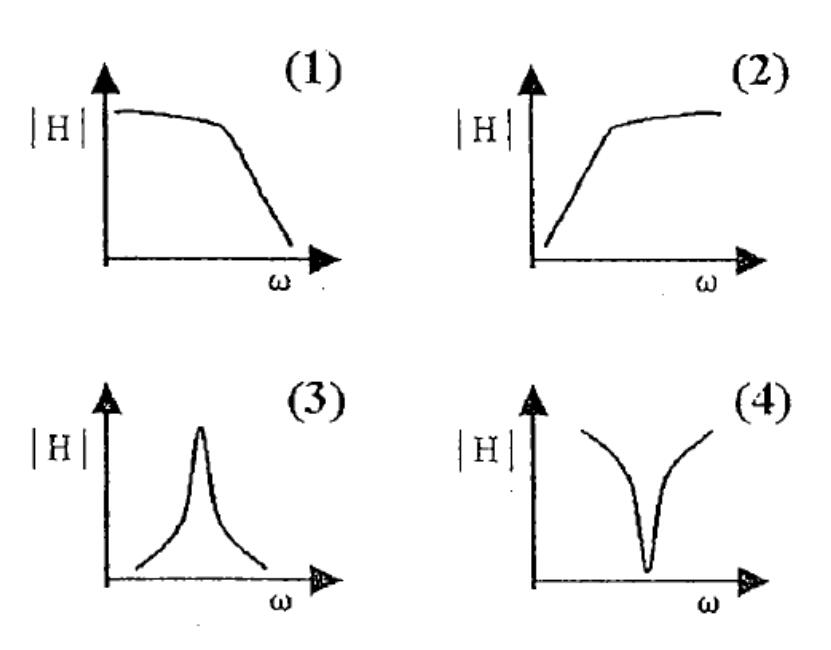
\includegraphics[width=.6\textwidth]{Figure1.jpg}
  \caption{(1): Low-Pass; (2): High-Pass; (3): Band-Pass; (4): Band-reject (also called band-stop or notch)}
  \label{img} 
\end{figure}
%--------------------------------- 

%---------------------------------
  \begin{figure}[H]
  \centering
  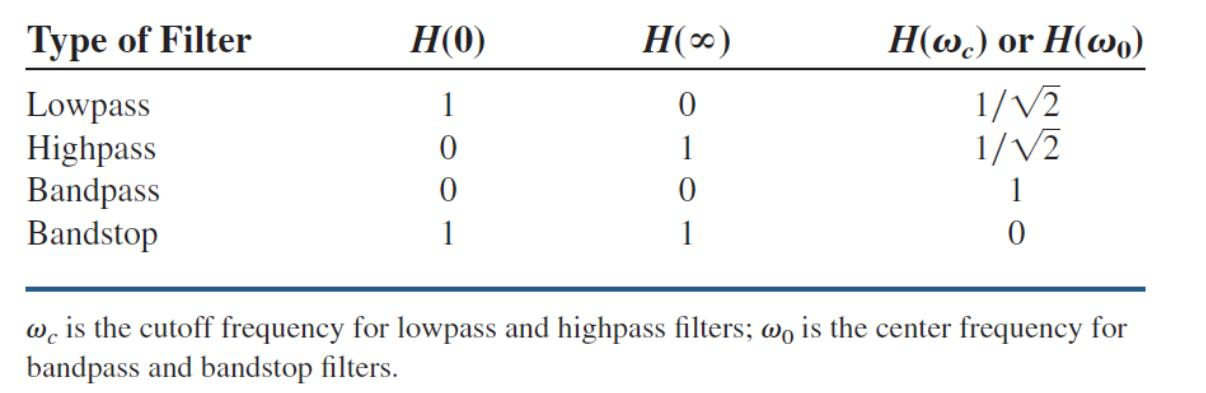
\includegraphics[width=.6\textwidth]{Figure2.jpg}
  \caption{Summary of the characteristics of ideal filters}
  \label{img} 
\end{figure}
%--------------------------------- 

Filter circuits, which you are going to build in this lab, contain resistors, capacitors, and inductors. They are all passive filters.
\subsection{High-Pass filter}
The high-pass filter we are going to build uses a capacitor and a resistor.
%---------------------------------
  \begin{figure}[H]
  \centering
  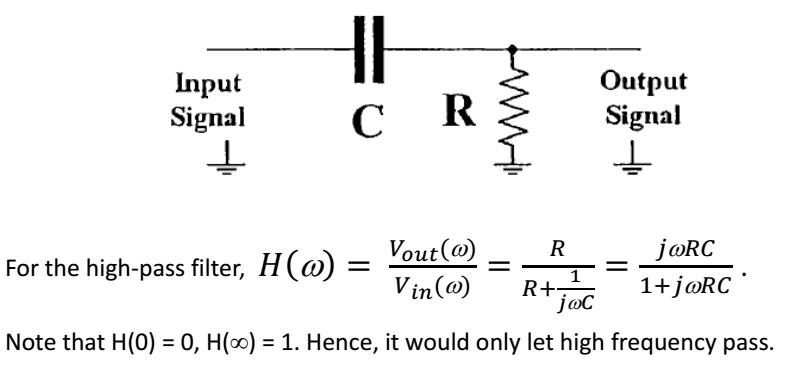
\includegraphics[width=.7\textwidth]{Figure3.jpg}
  %\caption{High-Pass filter}
  \label{img} 
\end{figure}
%--------------------------------- 
\subsection{Low-Pass filter}
The low-pass filter we are going to build uses a capacitor and a resistor.
%---------------------------------
  \begin{figure}[H]
  \centering
  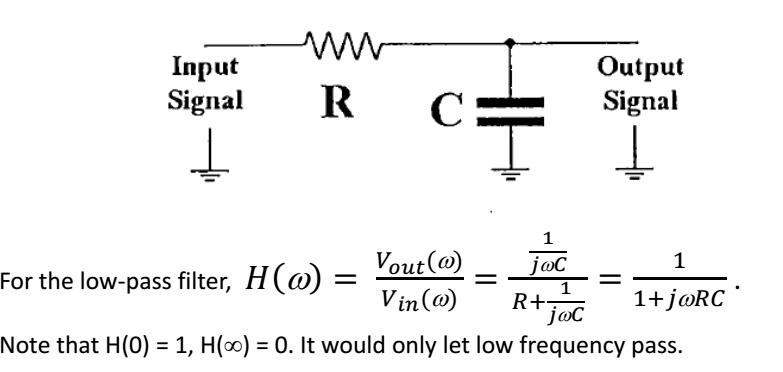
\includegraphics[width=.7\textwidth]{Figure4.jpg}
  %\caption{Low-Pass filter}
  \label{img} 
\end{figure}
%--------------------------------- 
\subsection{Band-Pass filter}
The band-pass filter we are going to build uses a capacitor, an inductor and a resistor.
%---------------------------------
  \begin{figure}[H]
  \centering
  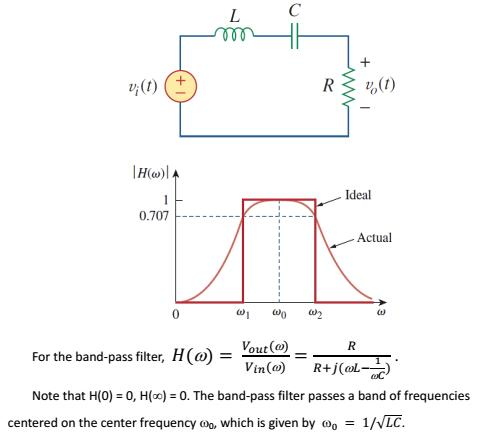
\includegraphics[width=.8\textwidth]{Figure5.jpg}
  %\caption{Band-Pass filter}
  \label{img} 
\end{figure}
%--------------------------------- 
\subsection{Band-Stop filter}
The band-stop filter we are going to build uses a capacitor, an inductor and a resistor.
%---------------------------------
  \begin{figure}[H]
  \centering
  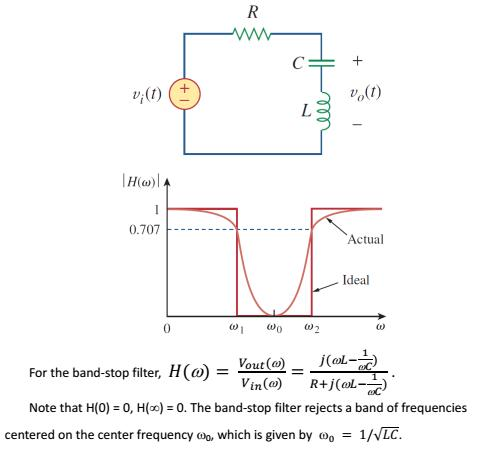
\includegraphics[width=.8\textwidth]{Figure6.jpg}
  %\caption{Band-Stop filter}
  \label{img} 
\end{figure}
%--------------------------------- 

\section{Results and Discussion}
\subsection{Low-pass Filter}
The measured data is listed below.
\begin{table}[H]
\centering
\begin{tabular}{|c|c|c|}
\hline
Frequency & Input signal amplitude, {[}Vppk{]} & Output signal amplitude, {[}Vppk{]} \\ \hline
1 MHz     & 9.6                                & 0.200                               \\ \hline
100 kHz   & 10.1                               & 0.237                               \\ \hline
50 kHz    & 10.3                               & 0.470                               \\ \hline
10 kHz    & 10.1                               & 2.21                                \\ \hline
5 kHz     & 10.1                               & 4.1                                 \\ \hline
1 kHz     & 10.7                               & 9.8                                 \\ \hline
500 Hz    & 10.7                               & 10.5                                \\ \hline
\end{tabular}
\caption{Measured data for low-pass filter}
\end{table}

The calculated data is listed below.
\begin{table}[H]
\centering
\begin{tabular}{|c|c|c|c|c|}
\hline
Frequency & \begin{tabular}[c]{@{}c@{}}Transfer\\  function\\  magnitude\end{tabular} & \begin{tabular}[c]{@{}c@{}}Expected\\  transfer\\  function\\  magnitude\end{tabular} & \begin{tabular}[c]{@{}c@{}}Transfer\\  function\\  magnitude\\ {[}dB{]}\end{tabular} & \begin{tabular}[c]{@{}c@{}}Expected\\ transfer\\  function\\  magnitude\\ {[}dB{]}\end{tabular} \\ \hline
1 MHz     & 9.6                                                                       & 0.020833                                                                              & 0.001621                                                                             & -33.6248                                                                                        \\ \hline
100 kHz   & 10.1                                                                      & 0.023465                                                                              & 0.016205                                                                             & -32.5915                                                                                        \\ \hline
50 kHz    & 10.3                                                                      & 0.045631                                                                              & 0.032397                                                                             & -26.8148                                                                                        \\ \hline
10 kHz    & 10.1                                                                      & 0.218812                                                                              & 0.159985                                                                             & -13.1986                                                                                        \\ \hline
5 kHz     & 10.1                                                                      & 0.405941                                                                              & 0.30835                                                                              & -7.83075                                                                                        \\ \hline
1 kHz     & 10.7                                                                      & 0.915888                                                                              & 0.851041                                                                             & -0.76315                                                                                        \\ \hline
500 Hz    & 10.7                                                                      & 0.981308                                                                              & 0.955561                                                                             & -0.16389                                                                                        \\ \hline
\end{tabular}
\caption{calculated data for low-pass filter}
\end{table}

The wave on the oscilliscope is shown below.
%---------------------------------
  \begin{figure}[H]
  \centering
  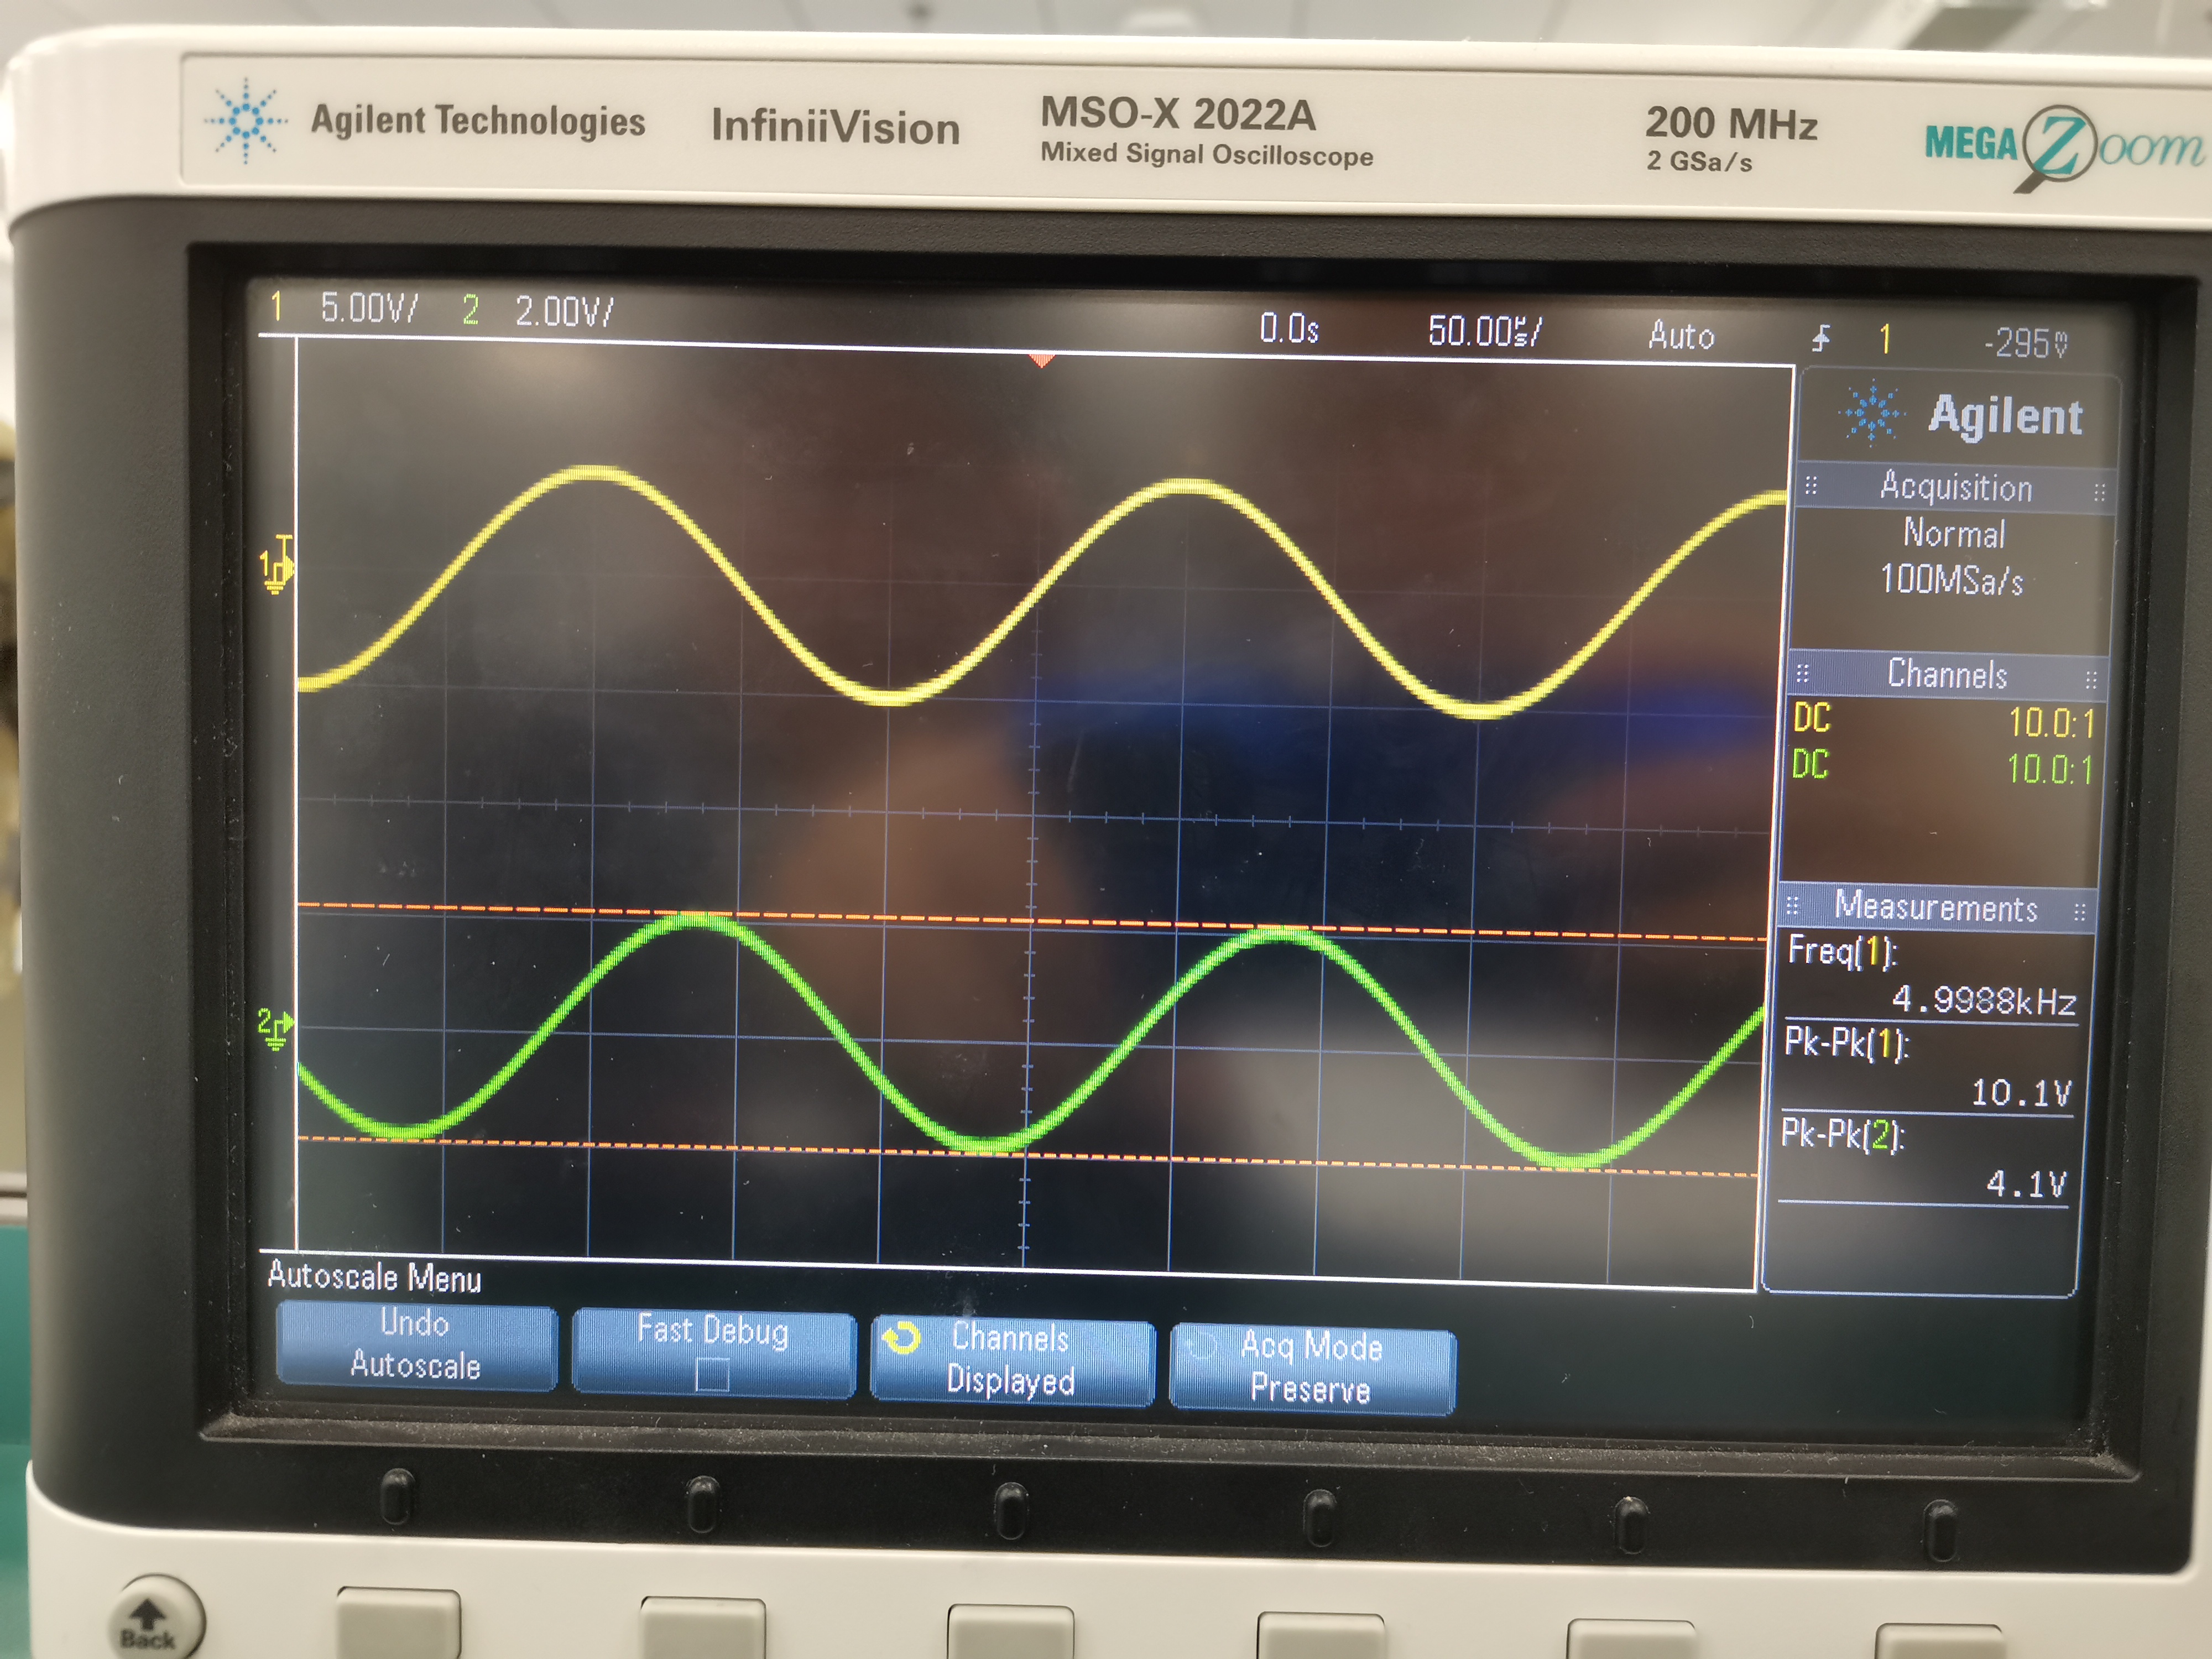
\includegraphics[width=.6\textwidth]{Figure7.jpg}
  \caption{Low-pass filter with frequency 5kHz}
  \label{img} 
\end{figure}
%--------------------------------- 

%---------------------------------
  \begin{figure}[H]
  \centering
  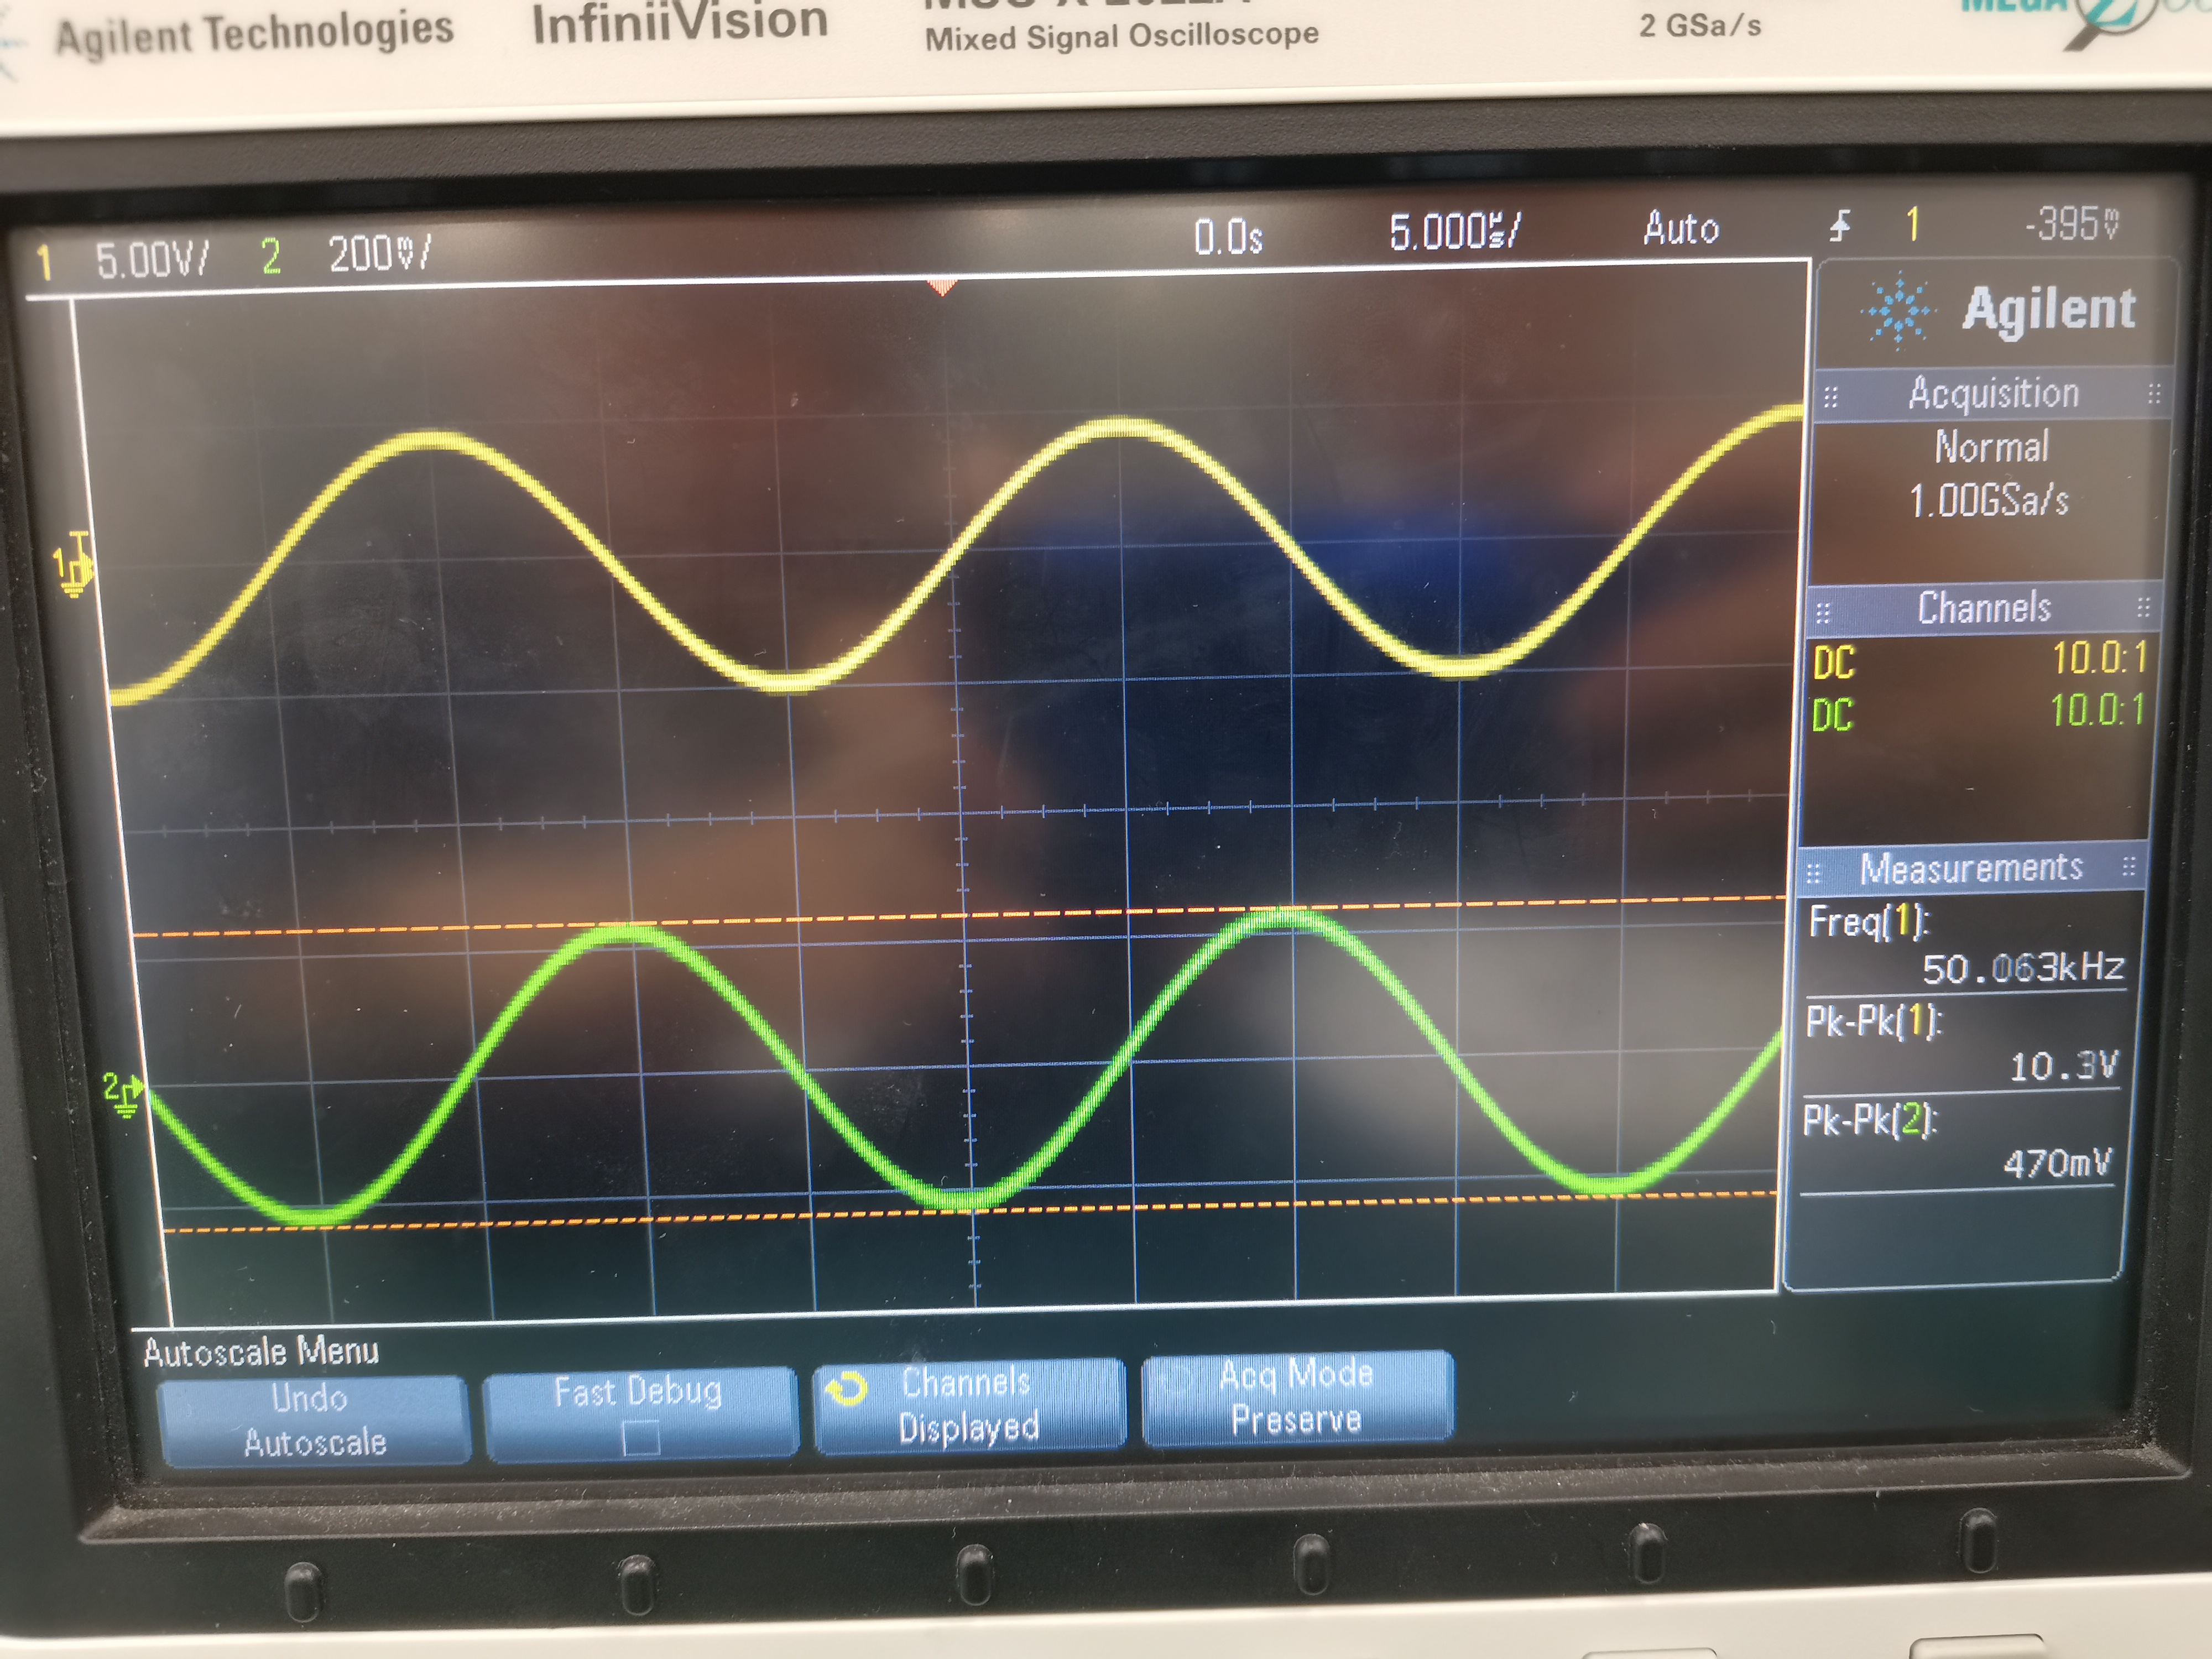
\includegraphics[width=.6\textwidth]{Figure8.jpg}
  \caption{Low-pass filter with frequency 50kHz}
  \label{img} 
\end{figure}
%--------------------------------- 


\subsection{High-pass Filter}
The measured data is listed below.
\begin{table}[H]
\centering
\begin{tabular}{|c|c|c|}
\hline
Frequency & Input signal amplitude, {[}Vppk{]} & Output signal amplitude, {[}Vppk{]} \\ \hline
1 MHz     & 9.6                                & 9.8                                 \\ \hline
100 kHz   & 10.1                               & 10.1                                \\ \hline
50 kHz    & 10.1                               & 10.1                                \\ \hline
10 kHz    & 9.8                                & 9.8                                 \\ \hline
5 kHz     & 9.2                                & 9.2                                 \\ \hline
1 kHz     & 4.2                                & 4.2                                 \\ \hline
500 Hz    & 2.29                               & 2.29                                \\ \hline
100 Hz    & 0.51                               & 0.51                                \\ \hline
\end{tabular}
\caption{Calculated data for high-pass filter}
\end{table}






The calculated data is listed below.
\begin{table}[H]
\centering
\begin{tabular}{|c|c|c|c|c|}
\hline
Frequency & \begin{tabular}[c]{@{}c@{}}Transfer\\  function\\  magnitude\end{tabular} & \begin{tabular}[c]{@{}c@{}}Expected\\  transfer\\  function\\  magnitude\end{tabular} & \begin{tabular}[c]{@{}c@{}}Transfer\\  function\\  magnitude\\ {[}dB{]}\end{tabular} & \begin{tabular}[c]{@{}c@{}}Expected\\ transfer\\  function\\  magnitude\\ {[}dB{]}\end{tabular} \\ \hline
1 MHz     & 1.02                                                                      & 1.00                                                                                  & 0.18                                                                                 & -1.1 × 10-5                                                                                     \\ \hline
100 kHz   & 1.00                                                                      & 1.00                                                                                  & 0                                                                                    & -0.00114                                                                                        \\ \hline
50 kHz    & 1.00                                                                      & 1.00                                                                                  & 0                                                                                    & -0.00456                                                                                        \\ \hline
10 kHz    & 0.97                                                                      & 0.99                                                                                  & -0.26                                                                                & -0.113                                                                                          \\ \hline
5 kHz     & 0.91                                                                      & 0.95                                                                                  & -0.81                                                                                & -0.434                                                                                          \\ \hline
1 kHz     & 0.40                                                                      & 0.52                                                                                  & -7.96                                                                                & -5.595                                                                                          \\ \hline
500 Hz    & 0.21                                                                      & 0.29                                                                                  & -13.4                                                                                & -10.61                                                                                          \\ \hline
\end{tabular}
\caption{Calculated data for high-pass filter}
\end{table}

The wave on the oscilliscope is shown below.
%---------------------------------
  \begin{figure}[H]
  \centering
  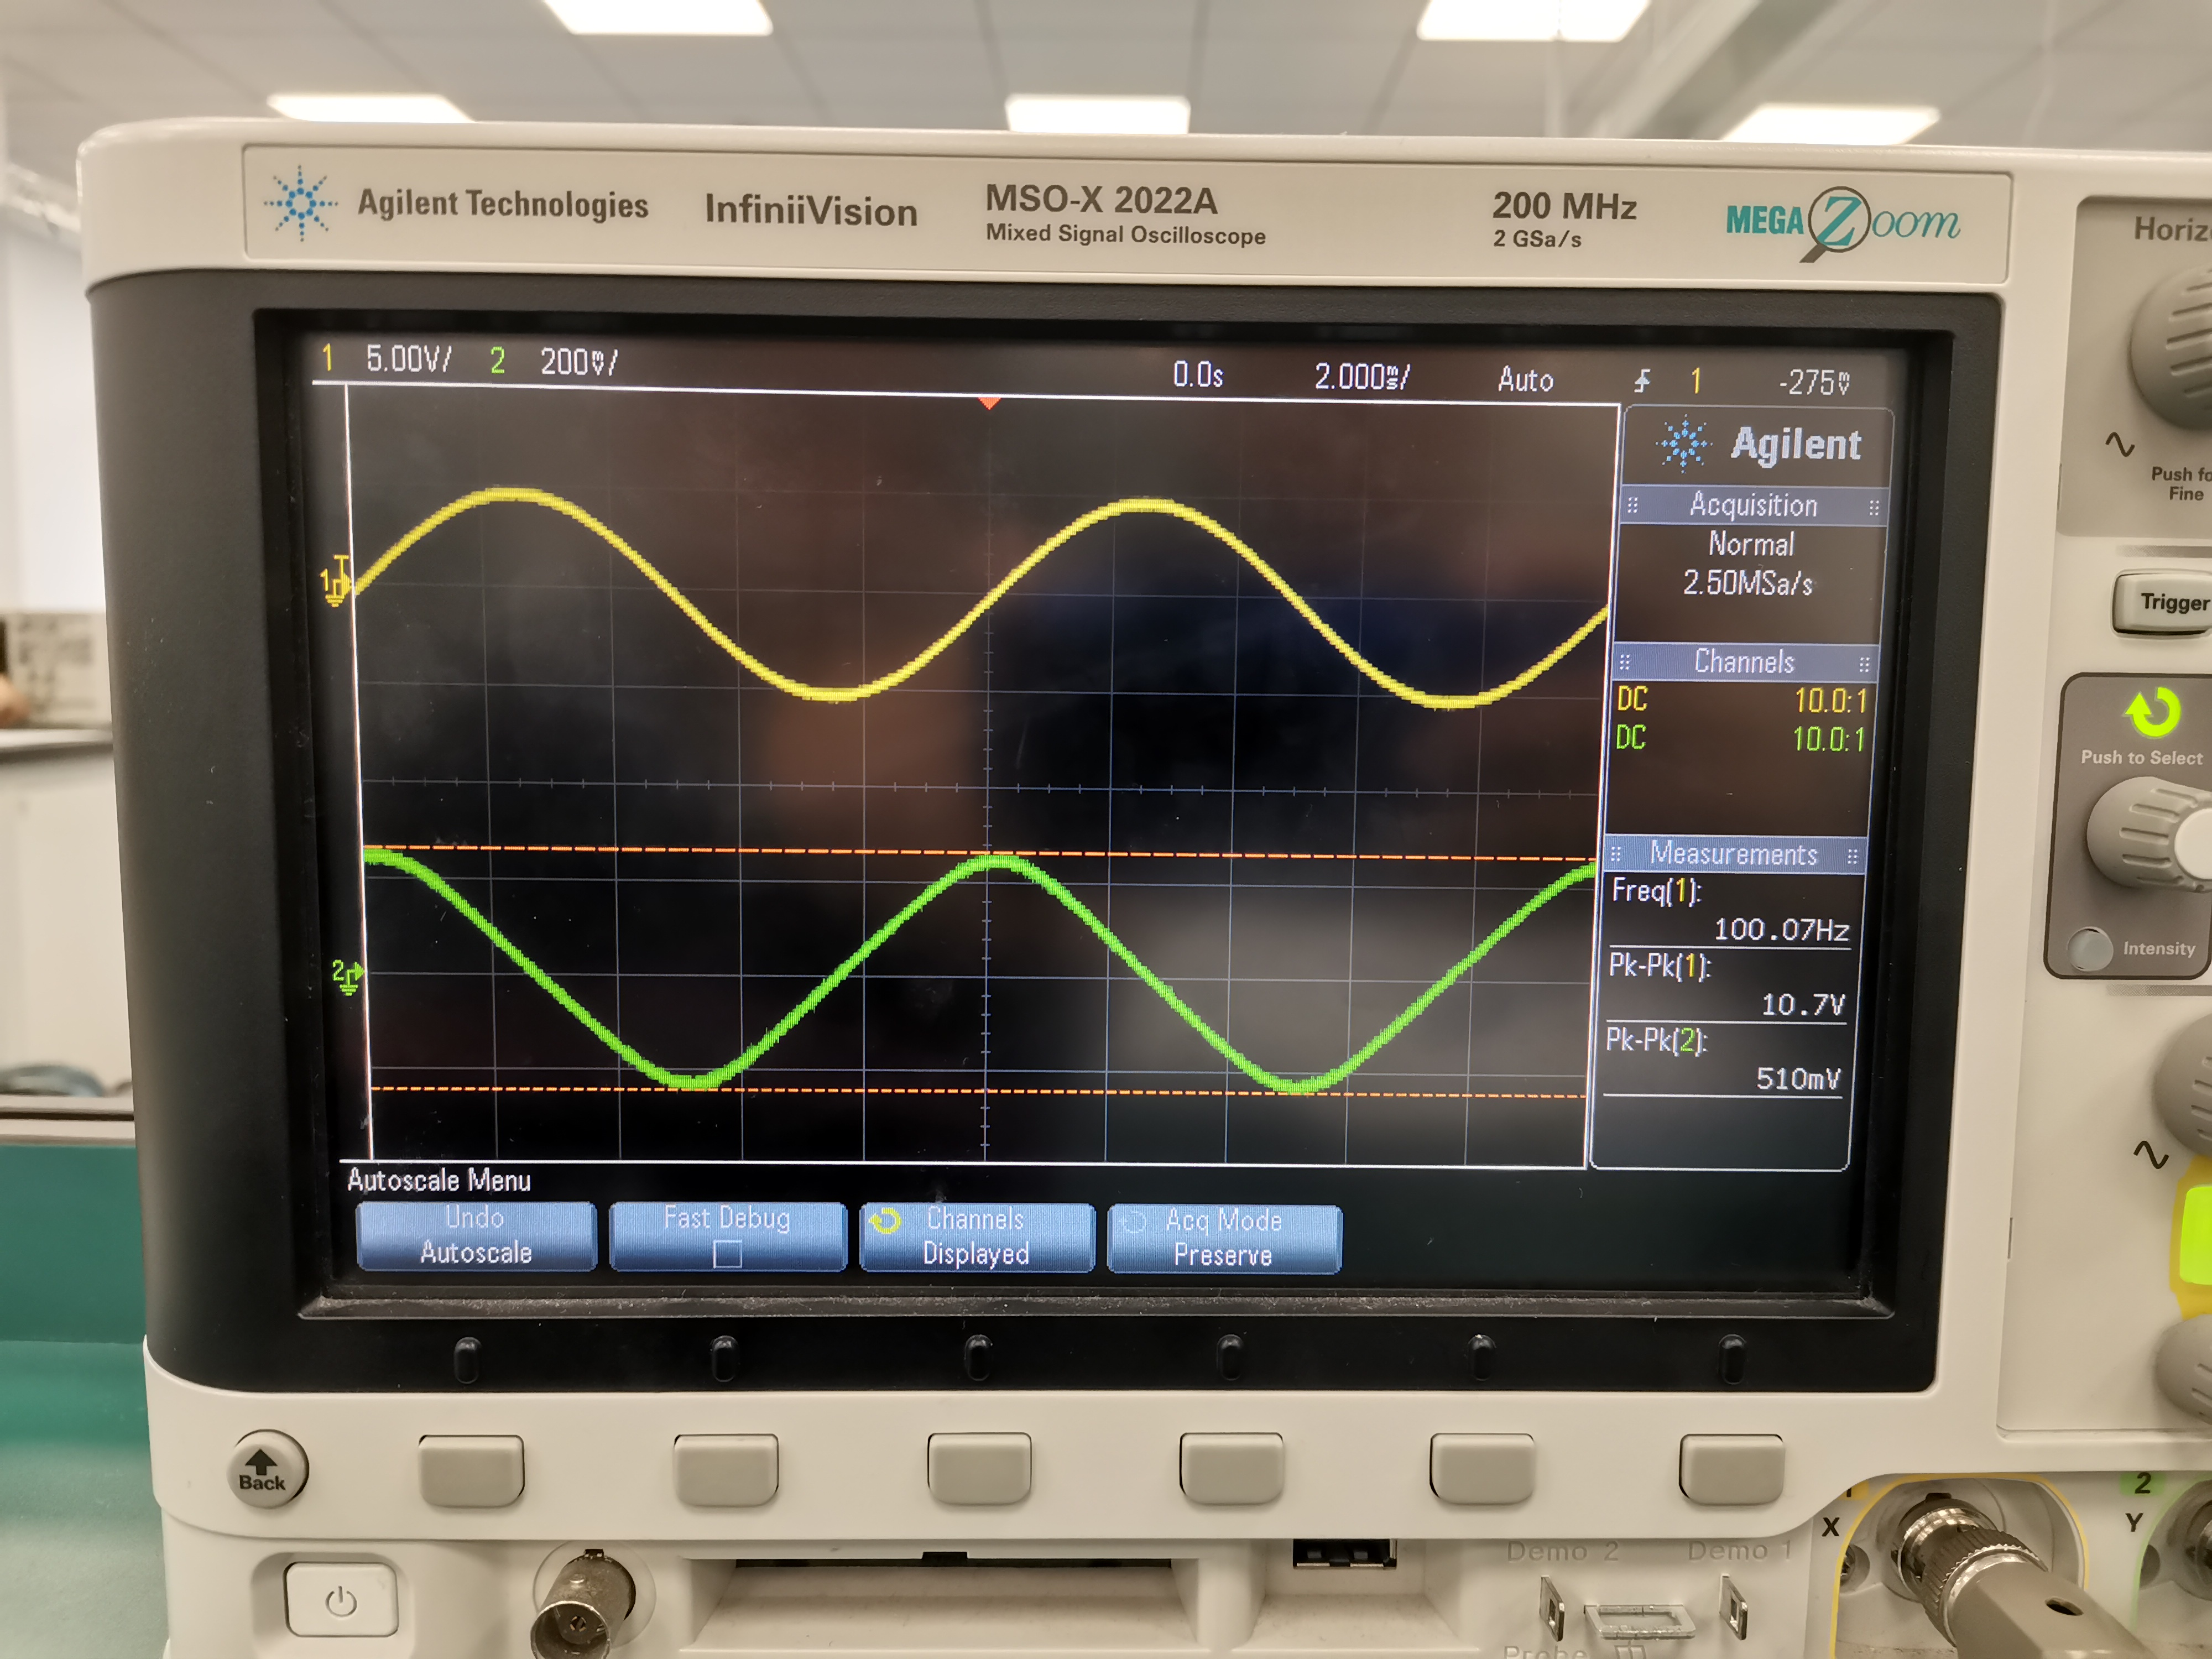
\includegraphics[width=.6\textwidth]{Figure9.jpg}
  \caption{High-pass filter with frequency 100Hz}
  \label{img} 
\end{figure}
%--------------------------------- 

%---------------------------------
  \begin{figure}[H]
  \centering
  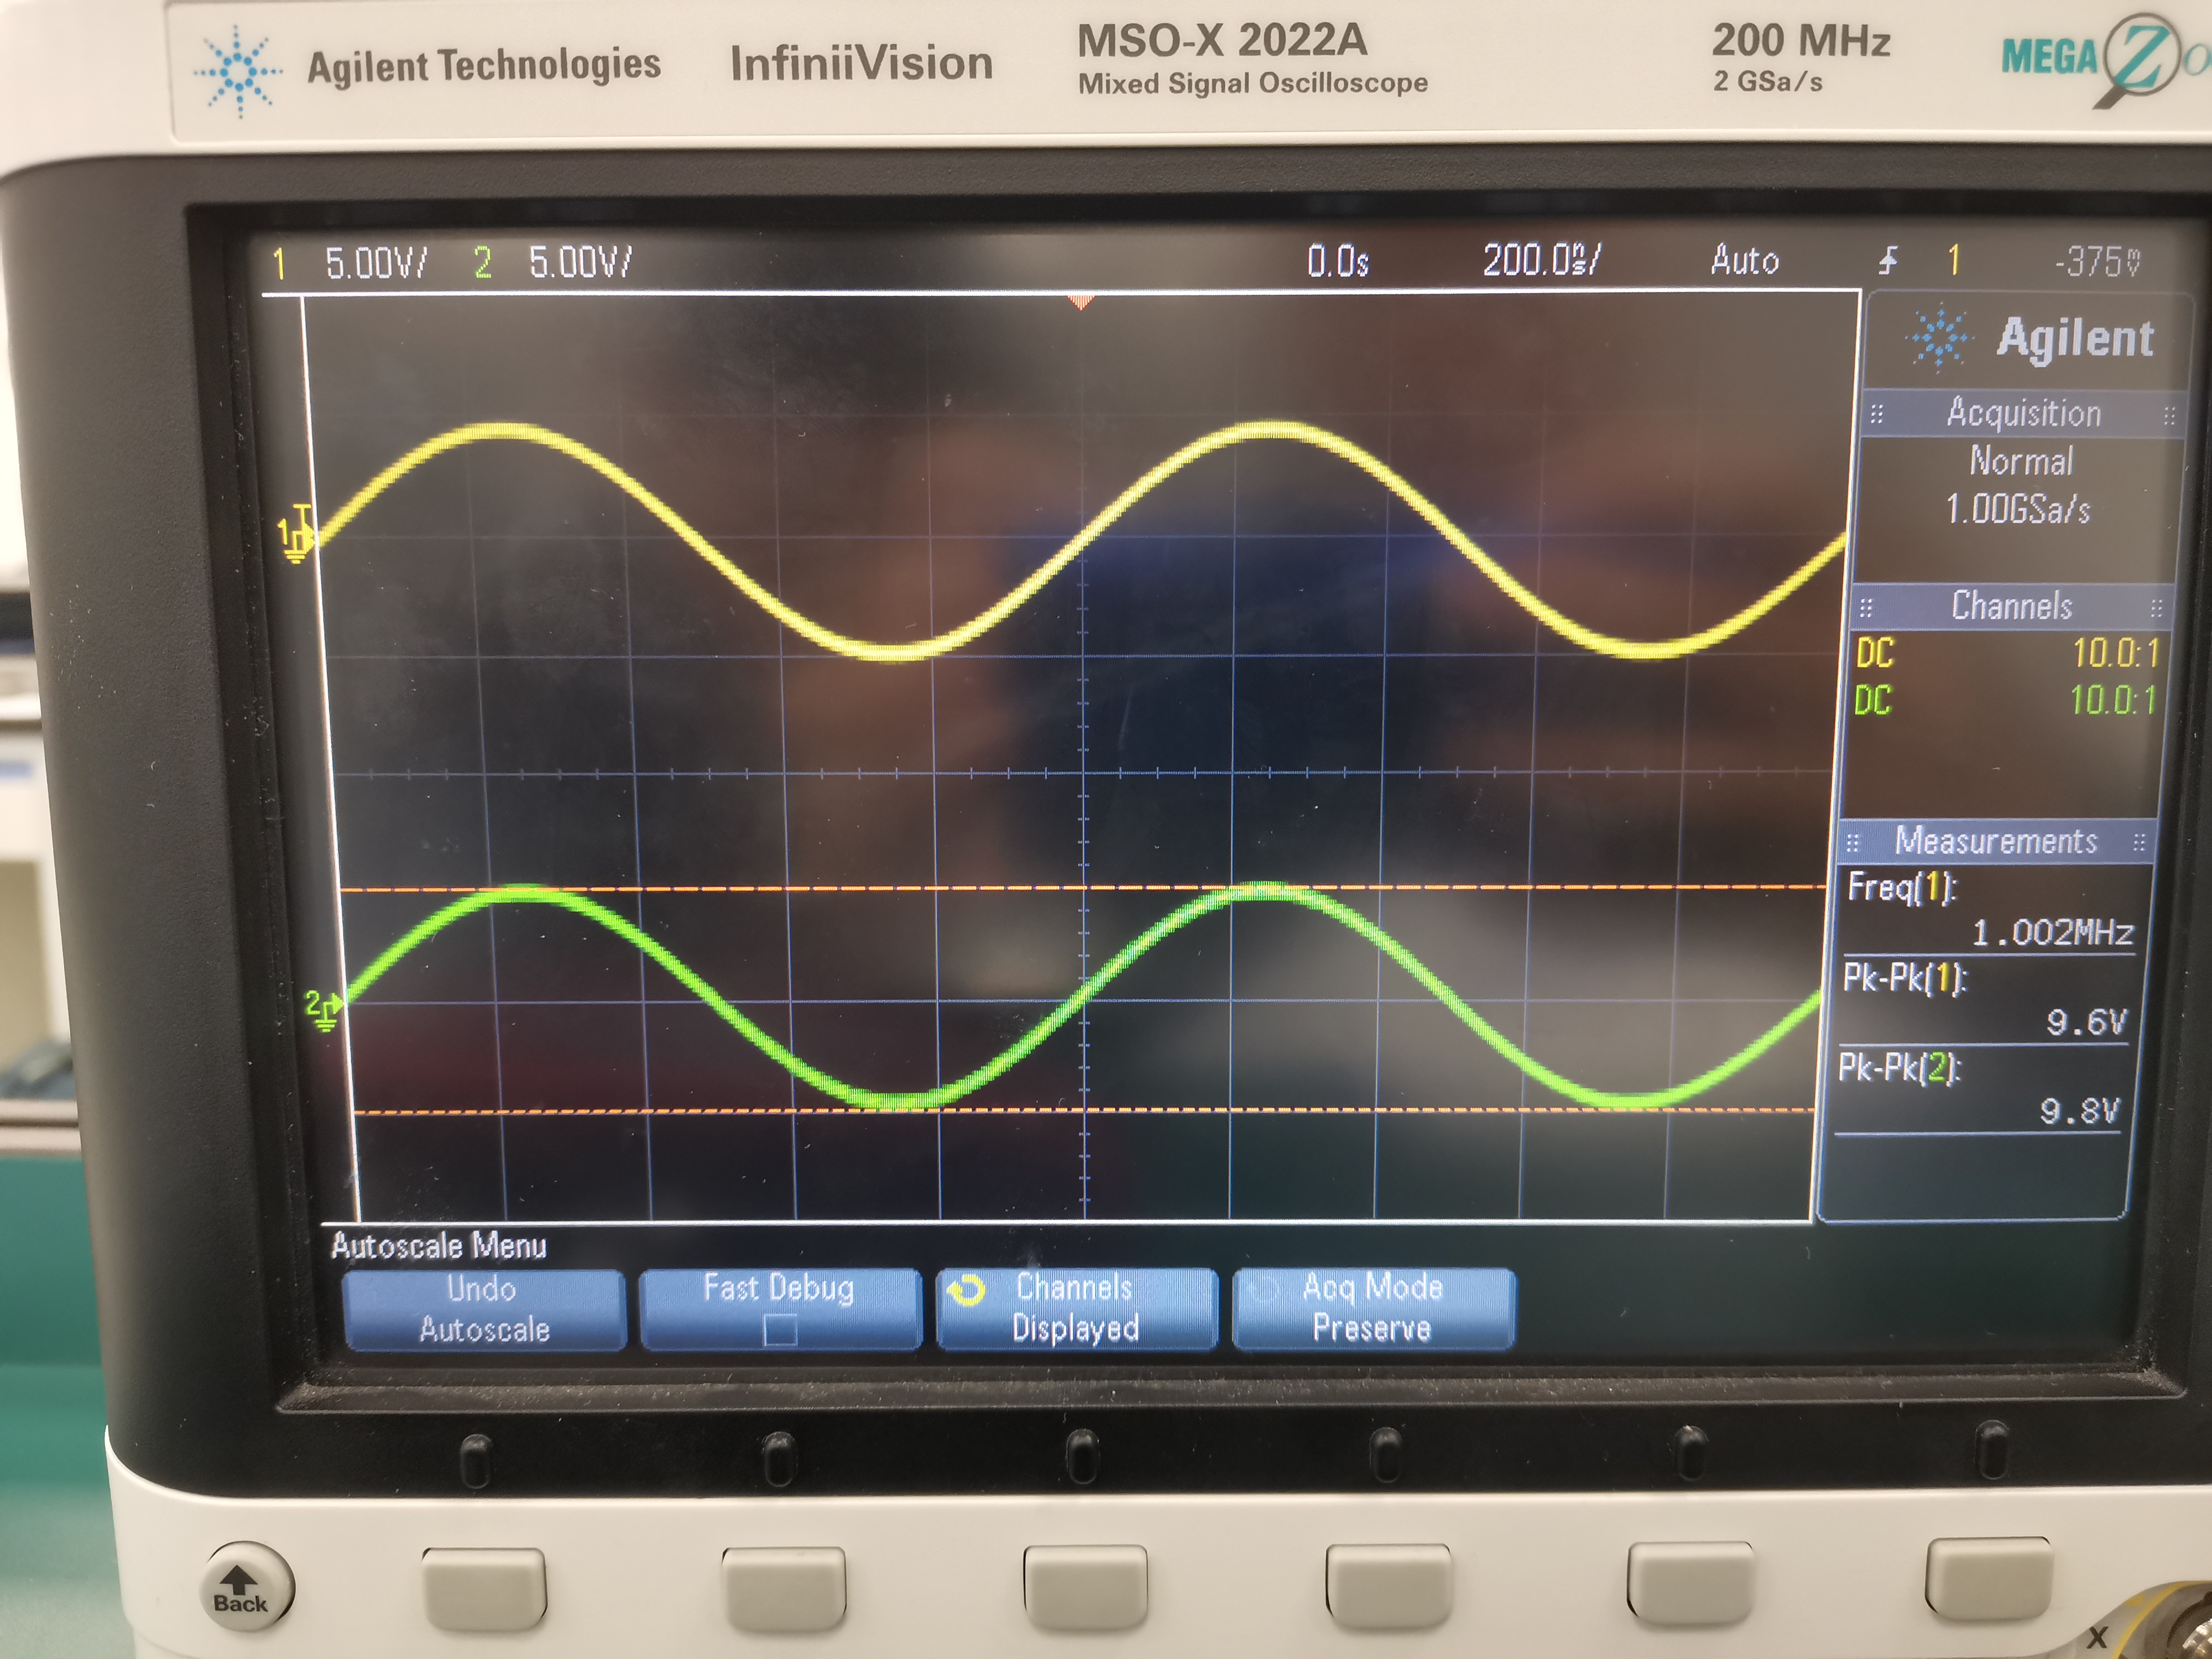
\includegraphics[width=.6\textwidth]{Figure10.jpg}
  \caption{High-pass filter with frequency 1MHz}
  \label{img} 
\end{figure}
%--------------------------------- 

\subsection{Band-pass Filter}
The measured data is listed below.
\begin{table}[H]
\centering
\begin{tabular}{|c|c|c|}
\hline
Frequency & Input signal amplitude, {[}Vppk{]} & Output signal amplitude, {[}Vppk{]} \\ \hline
1 MHz     & 10.3                               & 1.21                                \\ \hline
500 kHz   & 10.3                               & 3.02                                \\ \hline
100 kHz   & 10.3                               & 8.8                                 \\ \hline
50 kHz    & 10.1                               & 9.6                                 \\ \hline
10 kHz    & 10.1                               & 10.1                                \\ \hline
1 kHz     & 10.3                               & 4.2                                 \\ \hline
500 Hz    & 10.7                               & 2.33                                \\ \hline
\end{tabular}
\caption{Measured data for band-pass filter}
\end{table}

The calculated data is listed below.
\begin{table}[H]
\centering
\begin{tabular}{|c|c|c|c|c|}
\hline
Frequency & \begin{tabular}[c]{@{}c@{}}Transfer\\  function\\  magnitude\end{tabular} & \begin{tabular}[c]{@{}c@{}}Expected\\  transfer\\  function\\  magnitude\end{tabular} & \begin{tabular}[c]{@{}c@{}}Transfer\\  function\\  magnitude\\ {[}dB{]}\end{tabular} & \begin{tabular}[c]{@{}c@{}}Expected\\ transfer\\  function\\  magnitude\\ {[}dB{]}\end{tabular} \\ \hline
1 MHz     & 0.12                                                                      & 0.154                                                                                 & -18.60                                                                               & -16.224                                                                                         \\ \hline
100 kHz   & 0.29                                                                      & 0.299                                                                                 & -10.66                                                                               & -10.498                                                                                         \\ \hline
50 kHz    & 0.85                                                                      & 0.848                                                                                 & -1.37                                                                                & -1.427                                                                                          \\ \hline
10 kHz    & 0.95                                                                      & 0.961                                                                                 & -0.44                                                                                & -0.345                                                                                          \\ \hline
5 kHz     & 1.00                                                                      & 0.995                                                                                 & 0.00                                                                                 & -0.0416                                                                                         \\ \hline
1 kHz     & 0.41                                                                      & 0.527                                                                                 & -7.79                                                                                & -5.57                                                                                           \\ \hline
500 Hz    & 0.22                                                                      & 0.295                                                                                 & -13.24                                                                               & -10.60                                                                                          \\ \hline
\end{tabular}
\caption{Calculated data for band-pass filter}
\end{table}

%---------------------------------
  \begin{figure}[H]
  \centering
  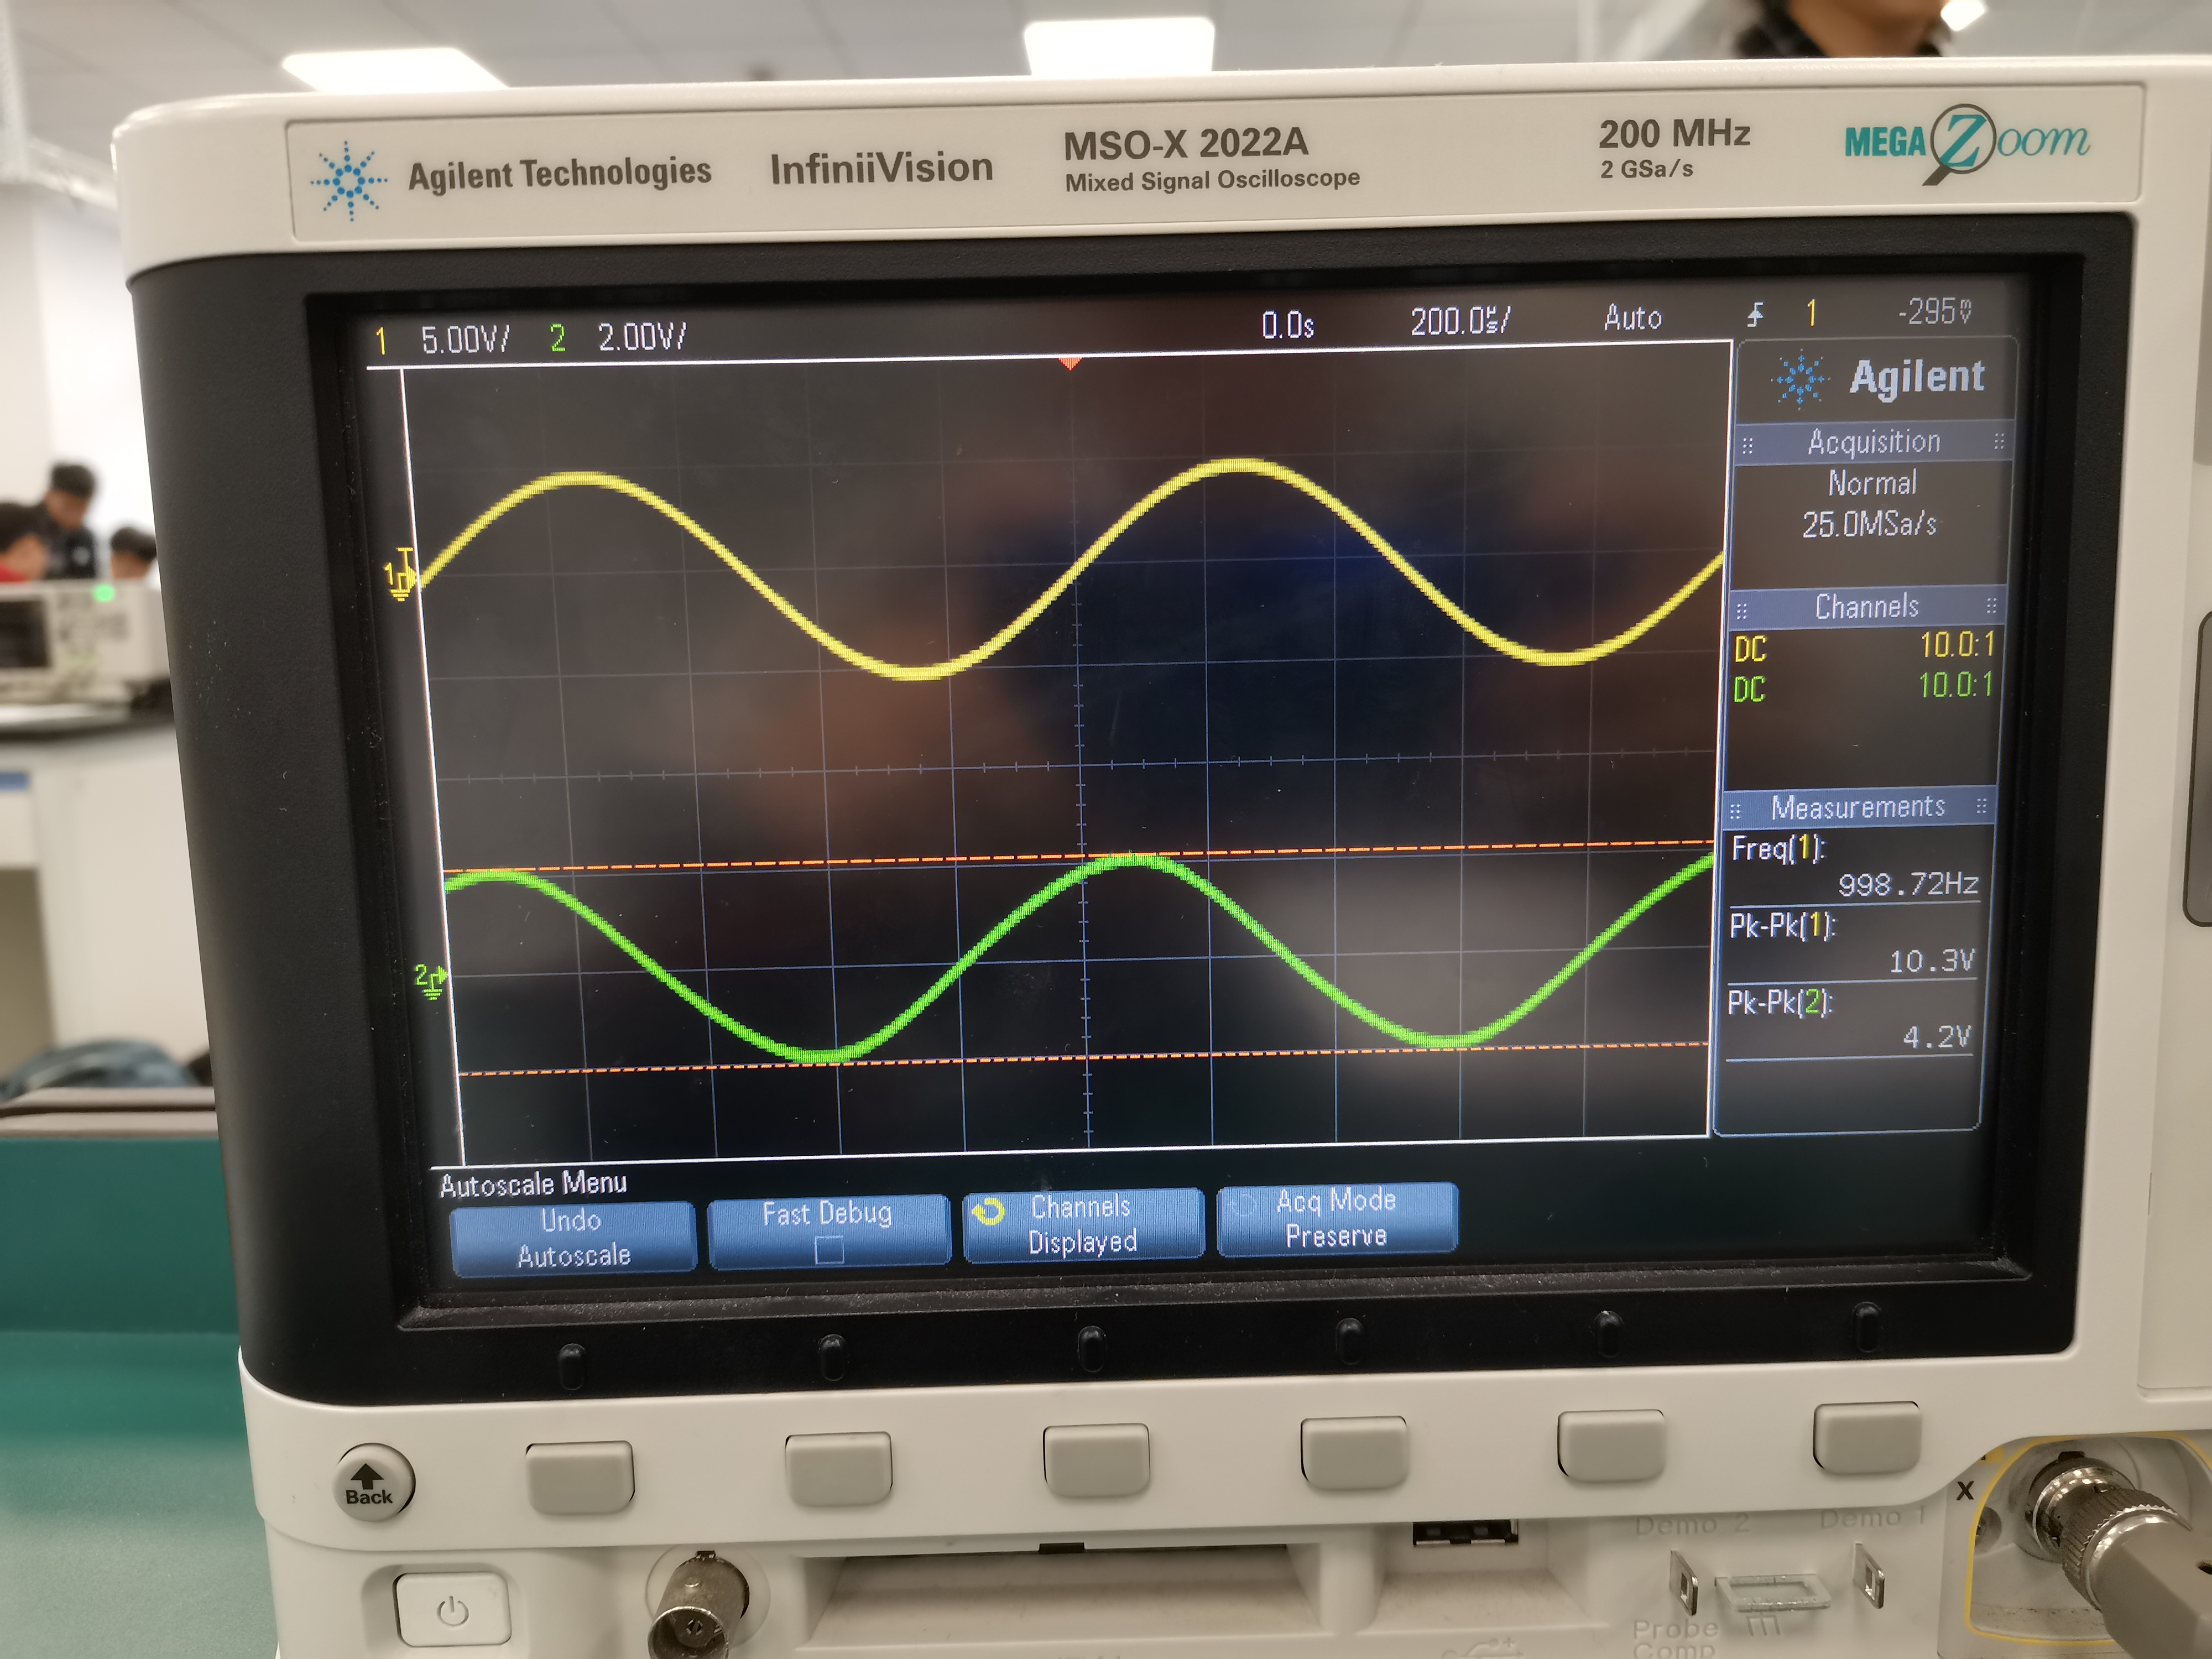
\includegraphics[width=.6\textwidth]{Figure11.jpg}
  \caption{Band-pass filter with frequency 1kHz}
  \label{img} 
\end{figure}
%--------------------------------- 

%---------------------------------
  \begin{figure}[H]
  \centering
  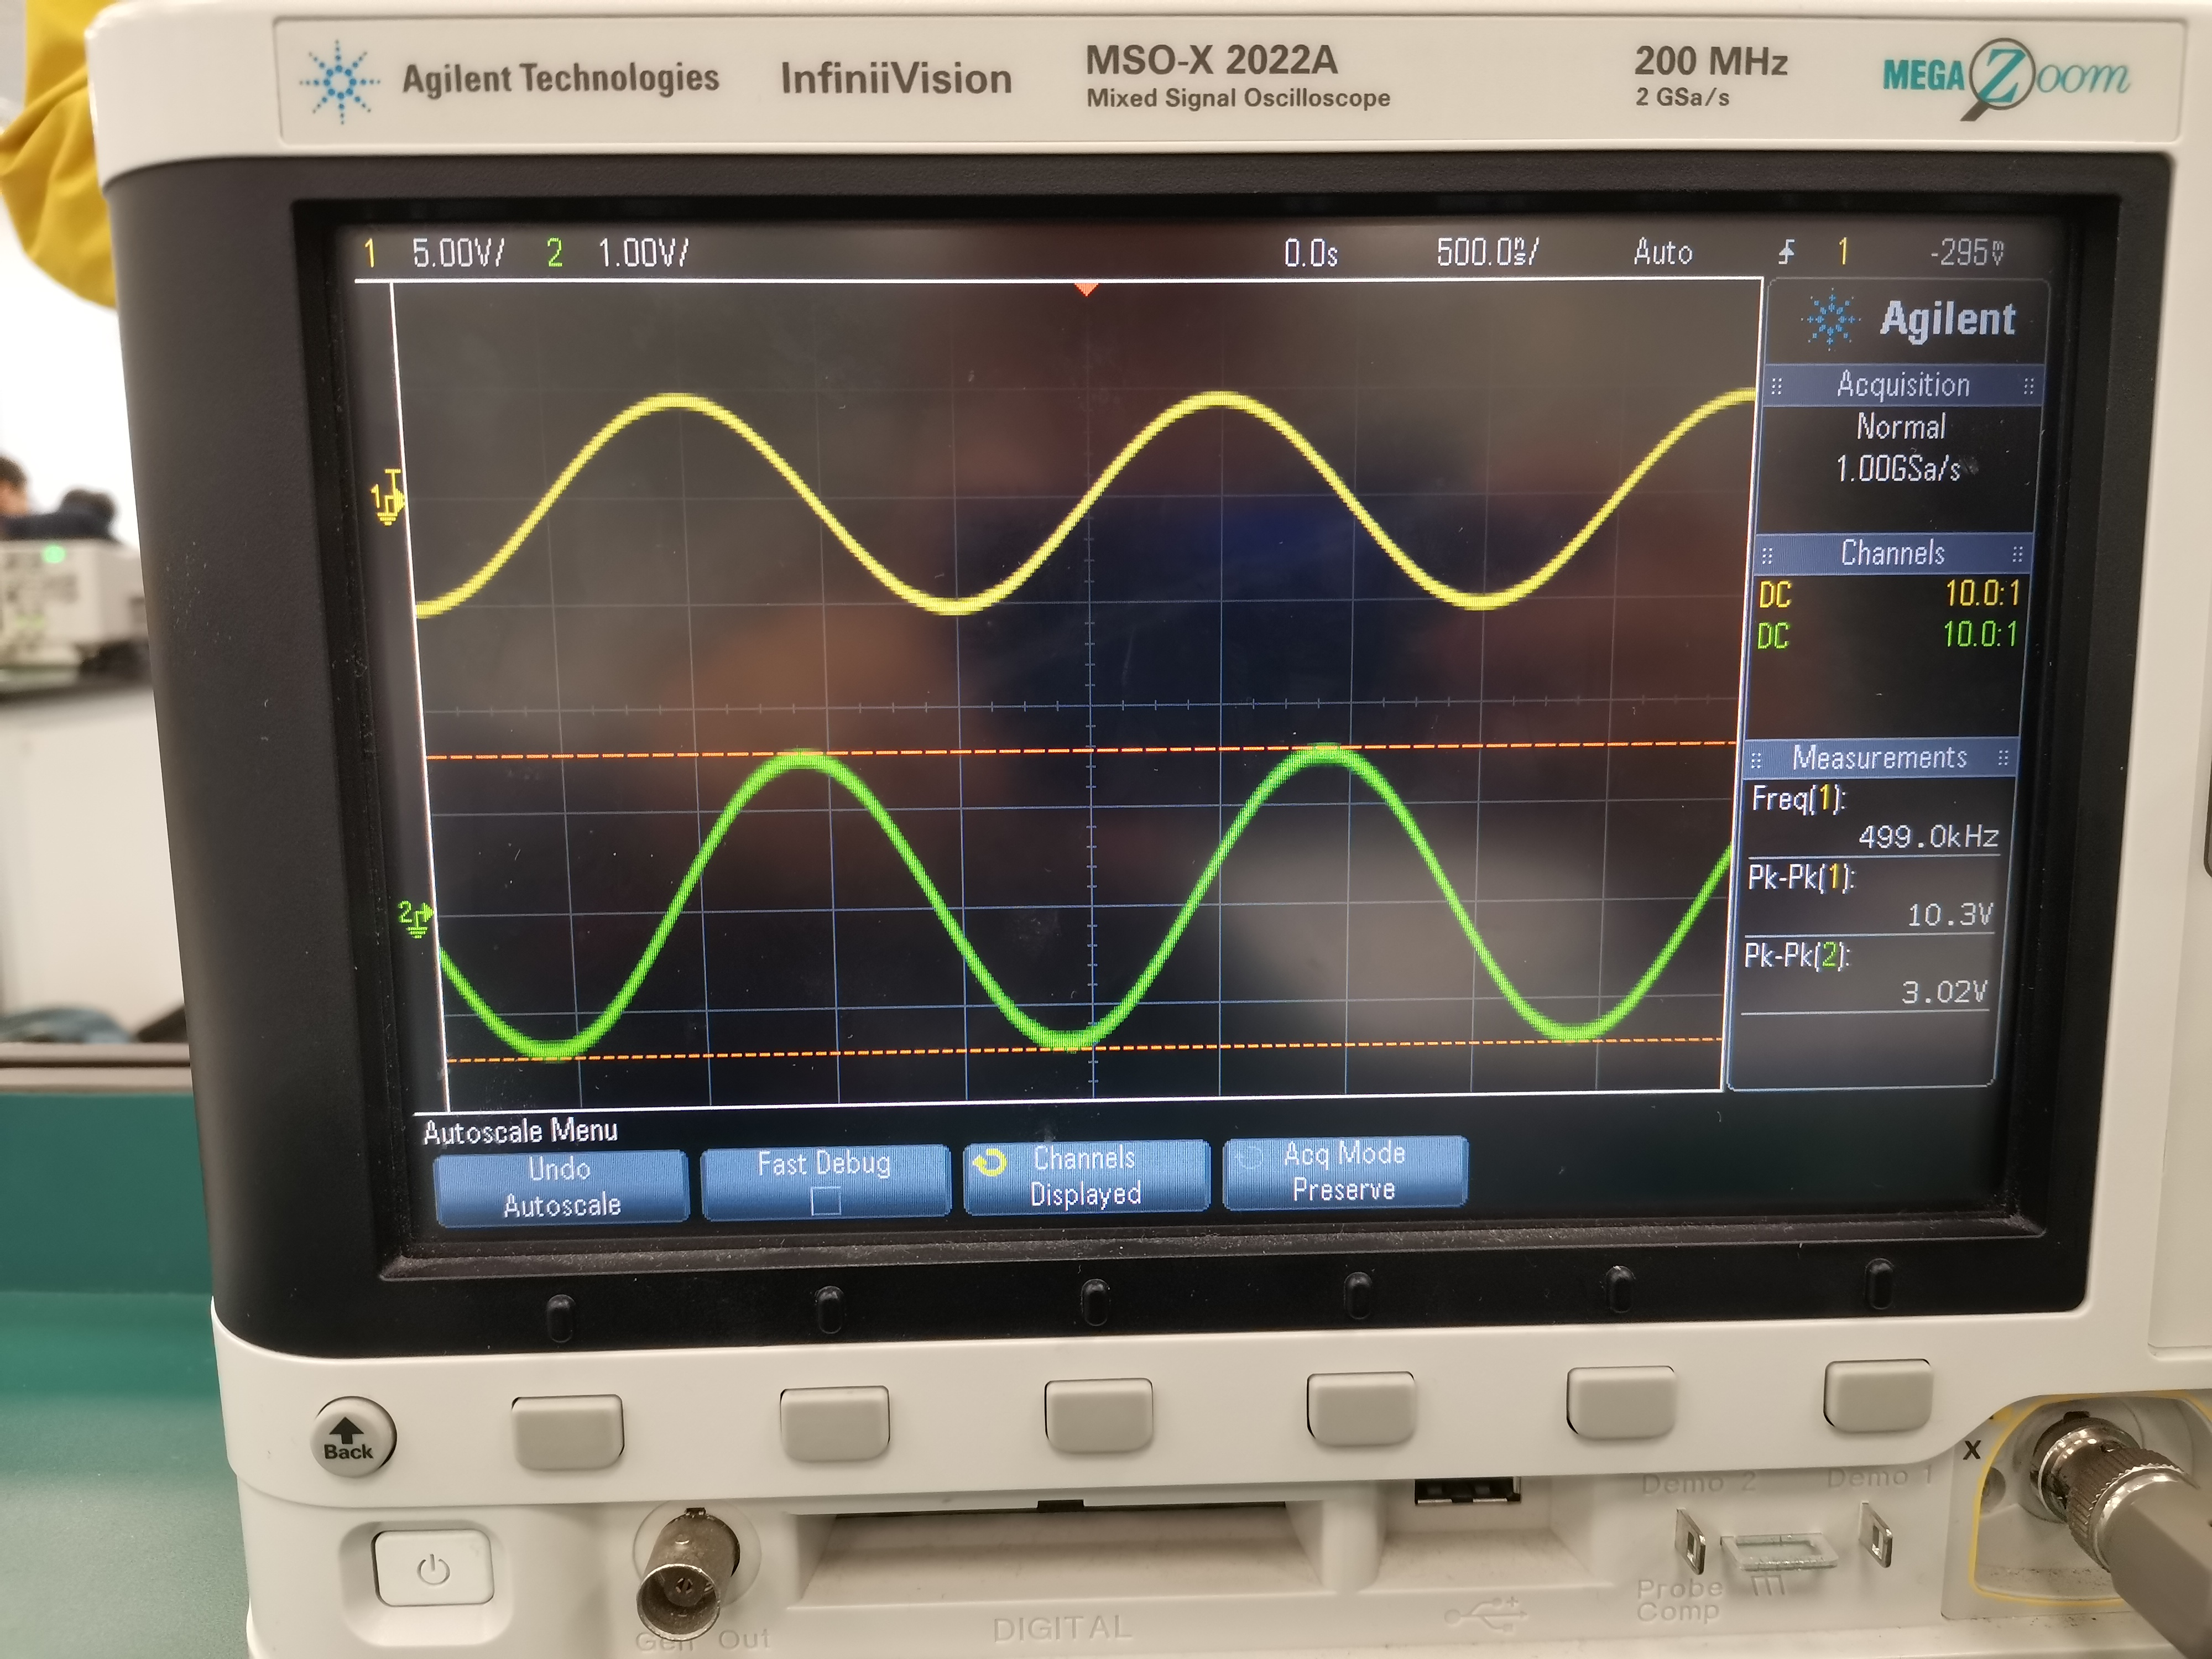
\includegraphics[width=.6\textwidth]{Figure12.jpg}
  \caption{Band-pass filter with frequency 500kHz}
  \label{img} 
\end{figure}
%---------------------------------

\subsection{Band-reject Filter}
The measured data is listed below.
\begin{table}[H]
\centering
\begin{tabular}{|c|c|c|}
\hline
Frequency & Input signal amplitude, {[}Vppk{]} & Output signal amplitude, {[}Vppk{]} \\ \hline
1 MHz     & 10.3                               & 10.3                                \\ \hline
500 kHz   & 10.3                               & 9.8                                 \\ \hline
300 kHz   & 10.3                               & 9.0                                 \\ \hline
200 kHz   & 10.3                               & 8.0                                 \\ \hline
100 kHz   & 10.3                               & 5.1                                 \\ \hline
50 kHz    & 10.1                               & 2.49                                \\ \hline
10 kHz    & 10.1                               & 1.67                                \\ \hline
5 kHz     & 10.3                               & 4.0                                 \\ \hline
1 kHz     & 10.5                               & 9.8                                 \\ \hline
500 Hz    & 10.7                               & 10.5                                \\ \hline
\end{tabular}
\caption{Measured data of band-reject Filter}
\end{table}

The Calculated data of the band-rejection filter is listed below.
\begin{table}[H]
\centering
\begin{tabular}{|c|c|c|c|c|}
\hline
Frequency & \begin{tabular}[c]{@{}c@{}}Transfer\\  function\\  magnitude\end{tabular} & \begin{tabular}[c]{@{}c@{}}Expected\\  transfer\\  function\\  magnitude\end{tabular} & \begin{tabular}[c]{@{}c@{}}Transfer\\  function\\  magnitude\\ {[}dB{]}\end{tabular} & \begin{tabular}[c]{@{}c@{}}Expected\\ transfer\\  function\\  magnitude\\ {[}dB{]}\end{tabular} \\ \hline
1 MHz     & 1.00                                                                      & 0.988                                                                                 & 0.00                                                                                 & -0.10                                                                                           \\ \hline
500 kHz   & 0.95                                                                      & 0.954                                                                                 & -0.43                                                                                & -0.41                                                                                           \\ \hline
300 kHz   & 0.87                                                                      & 0.886                                                                                 & -1.17                                                                                & -1.05                                                                                           \\ \hline
200 kHz   & 0.78                                                                      & 0.786                                                                                 & -2.19                                                                                & -2.09                                                                                           \\ \hline
100 kHz   & 0.50                                                                      & 0.529                                                                                 & -6.11                                                                                & -8.53                                                                                           \\ \hline
50 kHz    & 0.25                                                                      & 0.276                                                                                 & -12.16                                                                               & -11.17                                                                                          \\ \hline
10 kHz    & 0.17                                                                      & 0.098                                                                                 & -15.63                                                                               & -20.21                                                                                          \\ \hline
5 kHz     & 0.39                                                                      & 0.280                                                                                 & -8.22                                                                                & -11.04                                                                                          \\ \hline
1 kHz     & 0.93                                                                      & 0.850                                                                                 & -0.60                                                                                & -1.41                                                                                           \\ \hline
500 Hz    & 0.98                                                                      & 0.955                                                                                 & -0.16                                                                                & -0.40                                                                                           \\ \hline
\end{tabular}
\caption{Calculated data of the band-rejection filter}
\end{table}

%---------------------------------
  \begin{figure}[H]
  \centering
  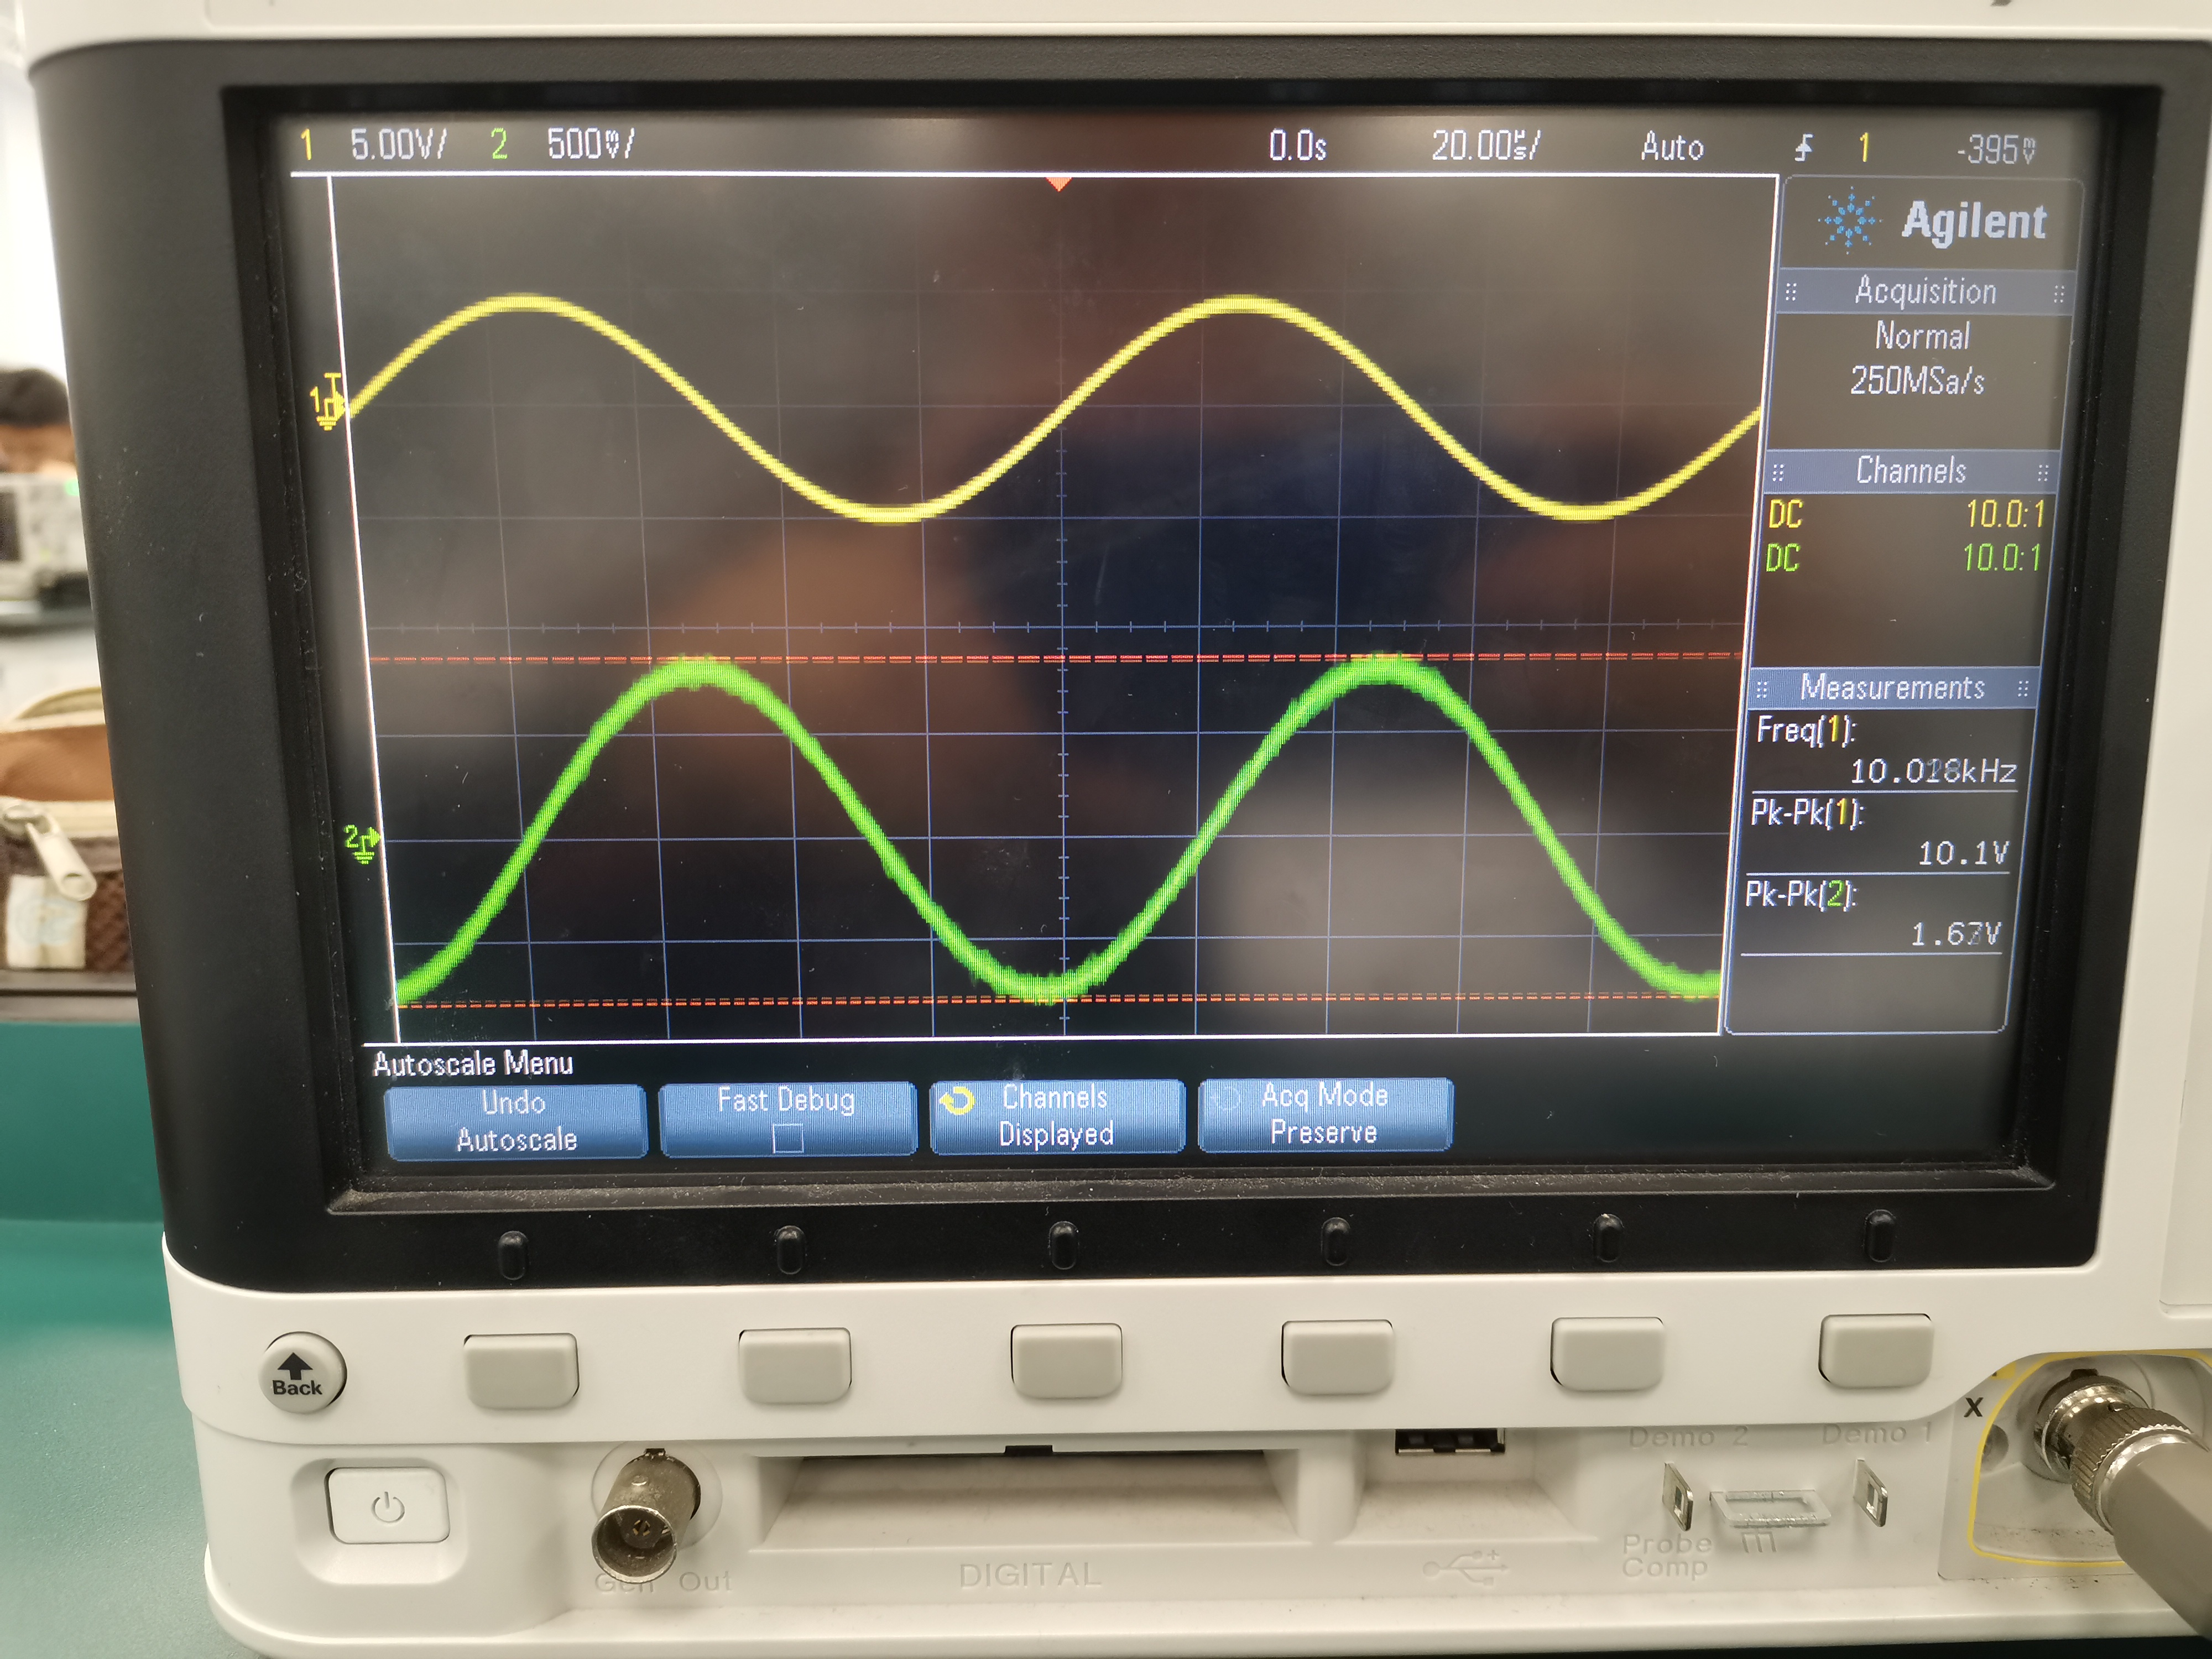
\includegraphics[width=.6\textwidth]{Figure13.jpg}
  \caption{Band-reject filter with frequency 10kHz}
  \label{img} 
\end{figure}
%--------------------------------- 

%---------------------------------
  \begin{figure}[H]
  \centering
  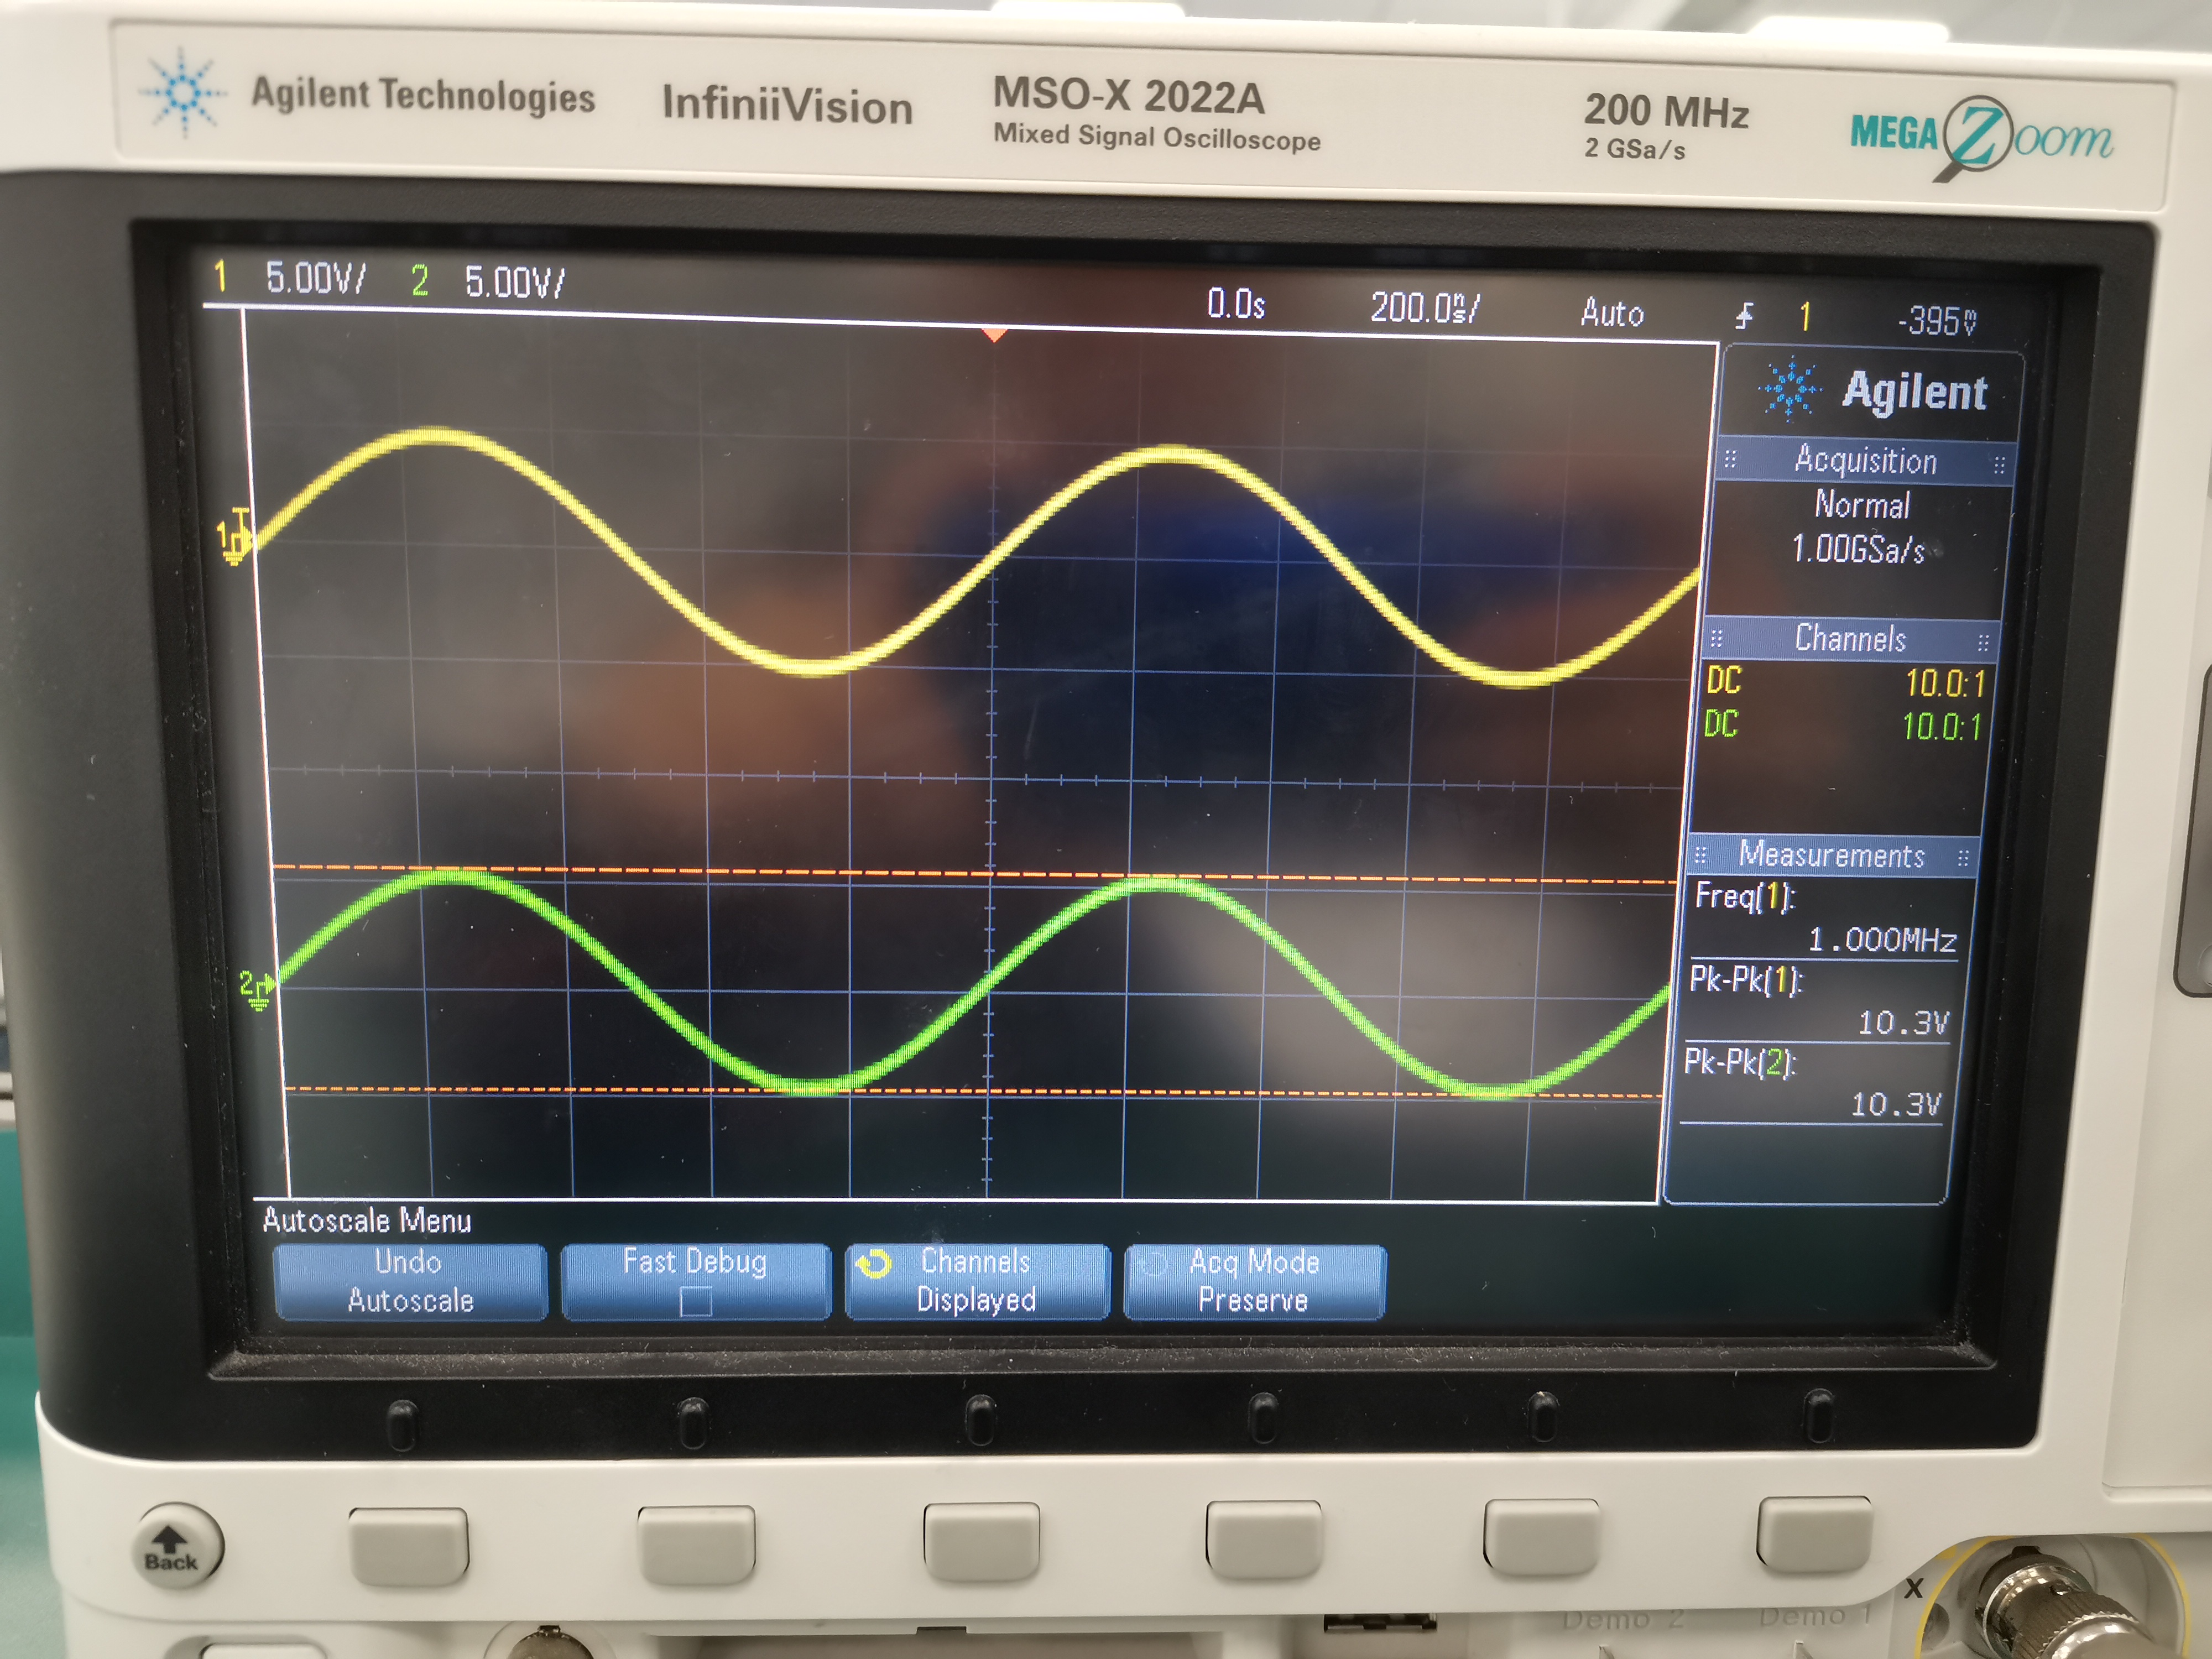
\includegraphics[width=.6\textwidth]{Figure14.jpg}
  \caption{Band-reject filter with frequency 1MHz}
  \label{img} 
\end{figure}
%---------------------------------

\section{Conclusion}
In this lab, we've learned about four types of filters – Low-Pass, High-Pass, Band-Pass, and Band-reject.\\

We also learned about transfer functions.\\

We predicted the theoretical result and make comparison with lab data.\\

In the tables of calculated data,we see that our transfer function magnitude and transfer funciton magnitude in dB is close to the expected value, which means our experiment is relatively successful.\\

One factor that may lead to inaccuracy is the wave on the oscilliscope is swinging so that we press the stop button and measure the value. So that in some cases, the position that we stop maybe far from the average position. 
\section{Reference}

Lab 5 Manual.



\section{Data sheet}



\end{document}



\end{document}